% Compile with: pdflatex (run TWICE to resolve cross-references), or paste into Overleaf.
\documentclass[11pt]{article}
\usepackage[letterpaper, margin=1in, top=0.9in, bottom=0.9in]{geometry}
\usepackage[T1]{fontenc}
\usepackage[utf8]{inputenc}
\usepackage{mathpazo}
\usepackage{microtype}
\usepackage[htt]{hyphenat}
\usepackage{amsmath}
\usepackage{amssymb}
\usepackage{titlesec}
\usepackage{enumitem}
\usepackage{booktabs}
\usepackage{graphicx}
\usepackage{caption}
\usepackage{subcaption}
\usepackage{float}
\usepackage[authoryear,round]{natbib}
\usepackage{hyperref}
\usepackage{xurl}
\usepackage{setspace}
\makeatletter
\renewcommand\@biblabel[1]{}
\makeatother

\titleformat{\section}{\normalfont\large\bfseries}{\thesection.}{0.6em}{}
\titleformat{\subsection}{\normalfont\normalsize\bfseries}{\thesubsection.}{0.5em}{}
\titlespacing*{\section}{0pt}{1.2em}{0.4em}
\titlespacing*{\subsection}{0pt}{0.9em}{0.25em}

\captionsetup{font=small, skip=4pt}

\setlength{\parskip}{0.55em}
\setlength{\parindent}{0pt}
\setlength{\emergencystretch}{3em}
\setlist{itemsep=0.2em, topsep=0.3em, partopsep=0pt, leftmargin=1.5em}

\begin{document}

% ─────────────────────────── TITLE PAGE ────────────────────────────────────
\begin{center}
  {\LARGE\bfseries Epic Games Store Giveaways:\\[0.3em]
   Causal Effect on Steam Player Engagement}\\[1em]
  {\large Nicholas Liu}\\[0.4em]
  {\normalsize 14.33 | Spring 2026}\\[0.4em]
  % {\small MIT Department of Economics}
\end{center}

\vspace{0.8em}
\hrule
\vspace{1em}

% ─────────────────────────── ABSTRACT ──────────────────────────────────────
\begin{center}
  \textbf{Abstract}
\end{center}

\noindent Does a free game giveaway on the Epic Games Store increase or decrease
engagement for the same title on Steam? Using a staggered difference-in-differences
event study across 446 treated games from 2018--2025, we find a two-phase dynamic.
In the giveaway month, Steam concurrent players rise by approximately 10--14\%, a
spike that is statistically significant under all three estimators (TWFE, LP-DiD,
stacked DiD) and survives a date-randomization placebo ($p<0.001$). The effect then
reverses; by month twelve the point estimates span roughly $0$ to $-23\%$, depending on
estimator. TWFE and LP-DiD produce large medium-run negatives, while
properly specified stacked DiD attenuates
to a near-zero estimate by the end of the window. A joint Wald test on the
pre-period event-study coefficients does not reject parallel trends at
conventional levels for the full sample but does
reject it for the low-traffic half of the panel, pointing to selection of
lifecycle-declining titles as a concern concentrated in smaller games.
We read the short-run spike as consistent with an advertising mechanism and the
medium-run negative estimates as an upper bound on any causal substitution effect
that is likely inflated by the continuation of pre-existing lifecycle decline in a
subset of selected titles.

\vspace{0.5em}
\noindent\textit{Keywords:} platform competition, cross-platform spillovers, video games, Epic Games Store, Steam

\vspace{1em}
\hrule
\vspace{1em}

% ─────────────────────────── 1. INTRODUCTION ───────────────────────────────
\section{Introduction}

When most gamers hear about a new video game, their first instinct is to open Steam and search for it.
This behavior reflects the social ecosystem Steam has cultivated: friend
lists, community hubs, reviews, achievements, and wishlist notifications so comprehensive
that it functions not only as a store but as the primary discovery and identity layer
for PC gaming. Even a game distributed \textit{entirely for free} on a rival platform is liable
to drive curious players to Steam first.

This intuition recently received vivid anecdotal support. In January 2026, Dave Oshry,
CEO of New Blood Interactive, publicly shared that when \textit{Blood West}, a 
first-person shooter published on Steam by New Blood, was given away for
free on the Epic Games Store over the 2025 holiday period, Steam sales surged by
approximately 200\% on the same day \citep{frvr2026}. ``I used to think EGS was a
Marketing Black Hole,'' Oshry wrote, ``but turns out having your game be free on Epic is
great advertising for Steam sales!'' The comment went viral in the gaming community,
sparking a Reddit thread on r/Steam that reached thousands of upvotes and generated
broad discussion about whether the Epic giveaway program systematically benefits Steam
engagement rather than draining it \citep{reddit2026}.

These observations raise an economically interesting causal question: does an
Epic Games Store free giveaway increase or decrease engagement for
the same game on Steam? Standard substitution logic predicts a decrease: a zero-price
substitute on a rival platform should divert players away from Steam. Yet the anecdotal
evidence points in the opposite direction, at least in the short run. The giveaway
may function as an advertising shock: it generates media coverage, social media chatter,
and word-of-mouth that raises awareness of the title and drives traffic to the platform
where players have their existing library, social graph, and community history: Steam.

The PC gaming platform market is a compelling context for this question. Steam,
operated by Valve and launched in 2003, remains overwhelmingly dominant with more than
120 million monthly active users and a catalogue exceeding 50{,}000 titles as of 2025.
Its competitive moat rests not only on library size but on thick social infrastructure:
forum discussions, user reviews, community guides, achievement tracking, and a friend-list
layer that creates switching costs no price cut can easily replicate. The Epic Games
Store (EGS), launched in December 2018 on the back of \textit{Fortnite}'s enormous
revenue, has pursued an aggressive free-game strategy as its primary differentiation
lever: since its launch, it has given away more than 400 games at no cost to users.
\citet{nabil2025} document that Steam significantly outperforms EGS in user-satisfaction surveys, 
suggesting that Epic's free game program does not close the platform quality gap.

Against this backdrop, this paper estimates the causal effect of EGS free giveaways on
Steam player engagement using a staggered difference-in-differences event study across
446 games given away between December 2018 and 2025. The identifying variation is the
timing of each game's first EGS giveaway: games awaiting future giveaways
serve as controls for currently treated games, exploiting the rolling staggered rollout
of the Epic program rather than relying on an external never-treated comparison group.
Engagement is measured via monthly average concurrent players scraped from SteamCharts.

To fix ideas, consider two games, both eventually given away by Epic, whose
giveaways fall eighteen months apart. In the absence of treatment, we would expect
their Steam player trajectories to follow similar paths once we condition on
calendar-month shocks common to all games. Comparing the earlier-treated game's
trajectory around its giveaway month, using the later-treated game as a not-yet-treated
control, identifies the causal effect of the promotion. Stacking such comparisons
across the eighty distinct treatment-month cohorts in the data traces out the full
event-study path from twelve months before to twelve months after treatment.

The central empirical finding is a two-phase dynamic. In the month of the giveaway and
the month after, Steam player counts rise by approximately 10--14\% in log terms, a
positive cross-platform spillover consistent with the advertising theory.
The contemporaneous spike is statistically significant ($p<0.001$) under all three
heterogeneous-treatment-robust estimators and passes a randomization placebo test.
The effect reverses within a few months of the giveaway, but how far it reverses is
estimator-dependent: TWFE and LP-DiD reach approximately $-11\%$ to $-27\%$ by month
twelve, while the preferred stacked-DiD specification (with stack-by-calendar-time
fixed effects) flattens to a statistically insignificant $+0.016$ by month twelve.
The spread across estimators bounds the medium-run causal substitution effect
between essentially zero and roughly $-23\%$; the true magnitude is almost certainly
closer to the lower end of this range because all three estimators are contaminated
to differing degrees by the pre-existing lifecycle decline of selected titles.
Repeat giveaways of the same game generate no detectable additional effect.

This pattern is consistent with three mechanisms operating at different time horizons.
First, the giveaway announcement attracts attention to the title on Steam, generating
a temporary engagement spike, consistent with an advertising mechanism.
Second, games selected for EGS giveaways may already be on a downward Steam
trajectory prior to treatment. The full-sample pre-period joint Wald test does not
reject parallel trends at the 5\% level ($F_{11,444}=1.72$, $p=0.067$), but the
point estimates drift downward toward $k=-1$, and a parallel test on the low-traffic
subsample does reject ($F_{11,213}=1.89$, $p=0.042$); the high-traffic subsample's
pre-period is statistically clean ($p=0.62$). Part of the observed post-giveaway
decline likely reflects this pre-existing trajectory in smaller titles continuing,
rather than a causal consequence of the giveaway.
Third, platform substitution where players migrate from Steam to their free
Epic copy may contribute a causal component. Because the medium-run
estimates span a wide range (from a non-significant $+1.6\%$ under stacked DiD to
$-27\%$ under TWFE), and because all three estimators absorb the lifecycle-decline
selection only imperfectly, the negative point estimates are best interpreted as an
upper bound on the magnitude of any true causal substitution effect.

The central contribution is the large-scale causal estimate of the full
dynamic trajectory of cross-platform spillovers from free game promotions (446 games,
38{,}641 game-month observations, seven years of giveaway history), including the
sustained post-giveaway reversal that prior work has not characterized.

The remainder of the paper is organized as follows. Section~\ref{sec:lit} reviews
related literature. Section~\ref{sec:data} describes the data and panel construction.
Section~\ref{sec:method} presents the empirical strategy. Section~\ref{sec:results}
reports results. Section~\ref{sec:discussion} interprets the findings and discusses
mechanisms. Section~\ref{sec:conclusion} concludes.

% ─────────────────────────── 2. LITERATURE REVIEW ──────────────────────────
\section{Literature Review}
\label{sec:lit}

\subsection{Cross-Platform Spillovers and Platform Competition}

The most directly related work is \citet{clarkson2025}, a doctoral dissertation whose
second chapter studies cross-platform spillover effects of gaming
platform giveaways. Using Steam player traffic data, Clarkson finds that games given
away by a competing platform (Epic) see Steam traffic increase by more than 24\%.
He also documents that word-of-mouth and Steam review activity increase significantly
during these promotions, and that spillover effects are larger for games that leverage
Steam-exclusive features (friend lists, achievements, community hubs) that are inaccessible
on the competing platform. The dissertation's question is nearly identical in spirit
to this paper, and its findings provide direct empirical support for a positive
cross-platform spillover mechanism.

This paper differs from Clarkson's in three respects. First, and most
substantially, Clarkson's analysis focuses on the contemporaneous effect;
this paper estimates the full twelve-month post-treatment trajectory using a
staggered DiD design with 446 games and seven years of giveaway history, documents
the systematic reversal below pre-giveaway baseline that prior work has not
characterized, and employs multiple heterogeneous-treatment-robust estimators
(LP-DiD, stacked DiD, Callaway--Sant'Anna) to bound the plausible range of the
causal effect. Second, by tracking the pre-period event-study path, this paper
provides evidence that the post-giveaway decline reflects selection on lifecycle
decline rather than causal substitution alone, a mechanism invisible to a
contemporaneous design. Third, the sample construction differs: Clarkson's
dissertation focuses on a curated subset of games, whereas this paper utilizes 
the full EGS giveaway catalogue.

More broadly, the question fits into the literature on platform competition and
multi-homing in two-sided markets \citep{rochet2003}. In two-sided
platforms, price cuts on one side (distributing games free to users) can strengthen
the platform's network if they attract more users and thereby make the platform more
attractive to developers. However, when two platforms primarily serve the same user base, 
as Steam and EGS do for PC gamers, a free promotion on one platform may simply reallocate 
engagement rather than expand the aggregate market.

\subsection{Network Effects and Social Multipliers on Gaming Platforms}

\citet{tudon2022} estimates the magnitude of direct network effects on Steam, and 
finds a 0.13\% own-demand increase per 1\% increase in friends' demand. 
This social-multiplier channel provides a mechanism for the advertising effect: 
by expanding the addressable player community, a free copy on a rival platform may activate
network complementarities that benefit the incumbent platform.

\subsection{Platform Satisfaction and Incumbency Advantage}

\citet{nabil2025} conduct a user-satisfaction survey comparing Steam and the Epic Games
Store, and find that Steam significantly outperforms EGS on content variety and ease of use, 
Their finding that Epic's free game program attracts users without closing the satisfaction
gap is consistent with a world where Steam's incumbency advantage is durable: players
who obtain a game via Epic may wish to still purchase the game on Steam to 
engage with Steam's ecosystem.

The observation that gamers treat Steam as their default discovery platform echoes the
insight from Adrian Chmielarz (creator of \textit{Painkiller} and \textit{Witchfire}):
``EGS is a shop, and Steam is a community. They don't have written reviews. They don't
have the forums. There's nothing to do there but to buy.'' \citep{frvr2026}. 
This functional asymmetry (Steam as a social community, EGS as a transactional storefront)
may explain why even free distribution via EGS can generate Steam traffic: the social
activity associated with a game such as discussion, reviews, and achievement hunting predominantly
occurs on Steam regardless of which platform delivered the copy.

\subsection{Staggered Difference-in-Differences Methodology}

The methodological backbone of the empirical strategy draws on 
\citet{cengiz2019} who introduce
stacked difference-in-differences, constructing cohort-specific balanced panels with
not-yet-treated controls and stacking them to obtain an event-study estimator free
of negative weights. \citet{dube2023} develop a local projections approach to DiD
event studies (LP-DiD) that is robust to heterogeneous treatment effects by restricting
each period-$k$ comparison to not-yet-treated controls. We also use \citet{callaway2021},
who establish that staggered treatment designs require cohort-specific estimands 
when treatment effects are heterogeneous across treatment cohorts. 
We use these methods as robustness checks on top of the standard TWFE estimator.

% ─────────────────────────── 3. DATA ───────────────────────────────────────
\section{Data}
\label{sec:data}

\subsection{Epic Giveaway History}

We obtained a Kaggle dataset \citep{dongre2025} recording every free game offered through
the Epic Games Store from December 2018 through 2025, comprising 541 giveaway events
corresponding to 471 unique game titles. The remaining 70 events are repeat appearances.
The source dataset flags repeat appearances with a ``(repeat)'' suffix appended to
the game name. Nine titles had this suffix incorrectly applied to their first
appearance; we manually corrected these so that
every title's earliest entry is flag-free and only genuine repeat giveaways carry the
``(repeat)'' suffix.

Repeats cluster in two distinct patterns: \textit{distant repeats}, where a game is
offered again more than twelve months after its first appearance (e.g., \textit{Kingdom
Come: Deliverance} at 57-month spacing), and proximate repeats, where the same
game is offered within a few months or even days of the first, most notably during
Epic's annual holiday giveaway batches.
Table~\ref{tab:epic_csv} summarizes the giveaway structure. We retain all giveaway dates
for each game to support the multi-event analysis.

\subsection{SteamCharts Monthly Player Data}

For each Epic giveaway title matched to a Steam App ID, we scraped monthly average and
peak concurrent player counts from \texttt{steamcharts.com/app/\{appid\}}. SteamCharts
renders its historical tables server-side, so standard HTTP requests suffice.
The overall panel spans July 2012 through February
2026, but each game's time series begins only from the month it first appeared on
SteamCharts (typically near its Steam release date). The median game has 88 months of data.

\subsection{Merge Pipeline}

Matching Epic game names to Steam App IDs requires reconciling inconsistent titling
(subtitles, punctuation, edition suffixes). We used RapidFuzz fuzzy string matching, 
which auto-matched 413 of 471 unique names; the remaining 58
received manual review, of which 50 were resolved to a valid Steam App ID and 8 were
confirmed absent from Steam (5 Epic exclusives and 3 placeholder entries).
Table~\ref{tab:pipeline} summarizes the pipeline. Fifteen matched entries are DLC packs
or in-game content releases mapped to the base game's Steam App ID; these are retained
but the measurement mismatch is discussed as a limitation.

\subsection{Final Panel and Summary Statistics}

The assembled dataset contains 38{,}642 game-month observations across 446 games.
One observation is subsequently dropped by the TWFE estimator as a singleton fixed
effect, leaving an effective regression sample of 38{,}641 game-months.
The outcome variable is $\ln(\texttt{avg\_players}+1)$, where \texttt{avg\_players}
is the SteamCharts monthly average concurrent player count. The $+1$ offset handles
months with zero reported players (common for low-traffic titles); the log transformation
compresses the heavy right tail driven by a small number of AAA titles.

Table~\ref{tab:sumstats} presents summary statistics. The raw player counts are highly
right-skewed: the mean monthly average of 1{,}584 players is more than 24 times the
median of 65 players, reflecting a distribution dominated by long-tail indie titles
with occasional blockbusters (e.g., GTA V, Destiny 2). The log-transformed outcome is
far better behaved (mean 4.43, SD 2.36). The repeat-event indicator is 1 in only 2\%
of game-month observations, reflecting that most games were given away exactly once.

Figure~\ref{fig:outcome} (left panel) shows overlaid density histograms of the
log-transformed outcome for pre-giveaway ($k < 0$) and post-giveaway ($k \geq 0$)
months. The post-giveaway distribution is shifted slightly leftward on average, but
the distributions are broadly similar in shape, with the heavy near-zero mass
reflecting the 101 games with a pre-treatment median below 10 concurrent players.
The right panel plots the unconditional mean of the outcome at each event-time
$k \in [-12, 12]$. In raw unconditional terms the pre-period mean is close to flat,
but this unconditional view does not difference out calendar-time shocks. A sharp uptick
is visible at $k = 0$, with partial persistence into $k = 1$ before declining.

Figure~\ref{fig:desc} provides three additional panels characterizing the panel's
structure. Panel (a) shows the pre-treatment distribution of log players across
the 429 games with a defined pre-treatment median (17 games with no pre-period
observations are omitted). Panel (b) shows that treatment cohorts are
broadly evenly distributed across 2019--2023, providing the timing variation needed
for staggered DiD identification. Panel (c) shows that roughly 10--15\% of games
in most cohort years received a repeat Epic giveaway at some point during the
panel; the plotted indicator is based on any repeat (proximate or distant), so
it exceeds the 30-game proximate-repeat count reported in
Table~\ref{tab:epic_csv}.

\subsection{Data Limitations}

Three data-source limitations bear on interpretation. First, SteamCharts reports
concurrent players, not purchases or unique installs; the giveaway effect on purchases
may be larger or differently timed than the player-count effect we estimate. Second,
fifteen matched events distributed DLC or in-game content rather than a standalone
base game; mapping these to the base game's App ID likely attenuates the estimated
treatment effect for those observations. Third, the dataset contains no genre
metadata, preventing a direct comparison of single-player versus multiplayer titles
within the current analysis, a distinction that matters because platform-switching
costs could differ substantially across those game types.

% ─────────────────────────── 4. EMPIRICAL METHOD ───────────────────────────
\section{Empirical Method}
\label{sec:method}

\subsection{Identification Strategy}

The identifying variation is the timing of each game's first Epic giveaway
across 80 distinct calendar months (aggregated to 29 quarterly cohorts for the
stacked DiD and Callaway--Sant'Anna estimators) spanning December 2018 through
late 2025. Because
the Epic program has cycled continuously through a broad catalogue of genres and
release-years, games awaiting future giveaways serve as natural controls for currently
treated games. 

An external never-treated control group was not constructed for two reasons.
First, building one would require scraping SteamCharts data for a large subset of
the approximately 50{,}000 titles on Steam that have never appeared in the EGS
catalogue, an undertaking infeasible without a principled sampling frame.
Second, any criterion for selecting which non-EGS games to include would
itself introduce selection bias: hand-picking games by genre, vintage, or
popularity to ``match'' the EGS catalogue risks assembling a control group
whose trajectories happen to be stable, biasing the comparison.
The not-yet-treated design sidesteps this problem because every game in
the sample is eventually treated by Epic, so the control group at any point is
drawn from the same population of EGS-eligible titles rather than from a
subjectively chosen external set. The limitations of this choice are discussed
in Section~\ref{sec:discussion}.

The key identifying assumption is parallel trends: in the absence of treatment, the
log player trajectory of games in different giveaway cohorts would have followed the
same path after conditioning on game and calendar-month fixed effects. This assumption
is more plausible if Epic's curation team does not systematically
select games at particular inflection points in their Steam life-cycle. There is,
however, reason to believe this assumption is at least partially violated. As documented
in Section~\ref{sec:results}, the pre-period event-study coefficients for $k \in [-12, -1]$
trace a negative slope, consistent with Epic preferentially selecting titles
already in lifecycle decline. This selection concern is the central identification caveat
of the design and implies that observed post-giveaway declines in Steam engagement may
partly reflect the continuation of a pre-existing downward trajectory rather than a
causal effect of the giveaway.

The assumption is partially testable. If parallel trends holds, the estimated
event-study coefficients for pre-treatment periods $k \in [-12, -2]$ should be
jointly indistinguishable from zero. We test this formally with a joint Wald
test of $H_0\colon \theta_k = 0$ for $k \in [-12,-2]$, constructed from the full
clustered covariance matrix of the TWFE coefficient vector. The full-sample
joint test does not reject parallel trends at the 5\% level but does reject at the 10\% level
($F_{11, 444} = 1.72$, $p = 0.067$). We supplement
the full pre-trend test with tests on the high and low traffic subsamples
(Section~\ref{ssec:pretrend}), which reveal that any pre-trend concern is
concentrated in smaller titles.

\subsection{Pooled TWFE Specification}

The primary specification is a two-way fixed-effects (TWFE) event-study regression on
the full unbalanced game-month panel:
\begin{equation}
\label{eq:pooled}
\ln(y_{it} + 1) = \alpha_i + \gamma_t +
  \sum_{\substack{k \in [-12,\,12] \\ k \neq -1}}
  \theta_k \cdot \mathbf{1}[\tilde{k}_{it} = k]
  + \varepsilon_{it}
\end{equation}
where $\alpha_i$ are game fixed effects, $\gamma_t$ are calendar-month fixed effects,
and $\tilde{k}_{it} = \text{clip}(k_{it},\,-12,\,12)$ is the event-time indicator
clipped to the $[-12, 12]$ window (observations outside the window are binned into the
endpoint cells). The omitted category is $k = -1$ (one month before the giveaway).
$\hat{\theta}_k$ estimates the average change in log Steam players at event-time $k$
relative to the pre-giveaway baseline, pooling first and repeat events per game.
Standard errors are clustered at the game level.

\textbf{Identification in a no-never-treated design.}
In settings where all units are eventually treated, event-time dummies can 
be near-collinear with calendar-month fixed effects if treatment is
concentrated in few periods. Here, the 80 treatment-month cohorts (equivalently,
the 29 treatment-quarter cohorts used by the stacked DiD and Callaway--Sant'Anna
estimators) are distributed across 80 distinct calendar months spanning December
2018 through late 2025, so at any calendar month $t$ the panel contains games at
a wide range
of event-times: some recently treated (small positive $k$), some approaching
treatment (small negative $k$), and some far from it (large $|k|$, clipped to
12). This within-calendar heterogeneity in event-time is what identifies the
calendar-month FE separately from the event-time dummies, and it is provided
entirely by the staggered timing structure rather than by an external never-treated
group. Omitting the single reference period $k = -1$ is therefore sufficient for
identification given the richness of the cohort spread.

\textbf{Boundary-bin clipping.}
Rather than restricting the estimation sample to the 336 games that have a full
$[-12, 12]$ observation window, we retain all 446 games by clipping event-time:
observations with $k < -12$ enter the $k = -12$ bin and observations with $k > 12$
enter the $k = 12$ bin. Restricting to full-window games would systematically
drop titles given away early in the EGS program (with little pre-treatment
history on SteamCharts) or very recently (with little post-treatment history). 
The cost of clipping is that the boundary-bin estimates at $k = -12$ and $k = 12$ pool observations
from multiple true event-times and should be read as averages over all periods
beyond the window, not single-period estimates.
As a robustness check, re-estimating Equation~\eqref{eq:pooled} on the 336-game
full-window subsample yields qualitatively identical results.

\subsection{Separated Specification: First vs.\ Repeat Giveaways}

To separate first-giveaway from repeat-giveaway effects, we add a scalar indicator
$\text{repeat\_event}_{it}$, equal to 1 in any month $t$ within 12 months after game
$i$'s \textit{second or later} giveaway:
\begin{equation}
\label{eq:separated}
\ln(y_{it} + 1) = \alpha_i + \gamma_t +
  \sum_{\substack{k \in [-12,\,12] \\ k \neq -1}}
  \beta_k \cdot \mathbf{1}[\tilde{k}_{it} = k]
  \;+\;
  \delta \cdot \text{repeat\_event}_{it}
  + \varepsilon_{it}
\end{equation}
$\beta_k$ isolates the first-giveaway causal effect; $\delta$ captures the average
incremental level shift from a repeat event holding the first-event trajectory fixed.
For the 33 games with a distant repeat ($>$12 months after the first), $\text{repeat\_event}_{it}
\equiv 0$ in the event window, so $\delta$ is identified primarily by the 30 games with
a proximate repeat. For micro-batch repeats with gaps under one month (e.g., \textit{Escape
Academy} re-offered within days during the 2023--2024 holiday batch), the cluster is
collapsed to its earliest date and treated as a single event. A simpler alternative
is to exclude all 30 proximate-repeat games from the analysis entirely; given that
they constitute less than 7\% of the sample and the repeat-event estimate is
indistinguishable from zero. The clean-sample robustness check
(Appendix~\ref{app:robustness}) confirms this exclusion leaves main estimates
unchanged.

\subsection{Robustness Estimators}

We employ three complementary robustness estimators.
Because treatment timing is staggered across six years, the standard TWFE estimator
is potentially biased when treatment effects are heterogeneous across cohorts
\citep{callaway2021}. TWFE remains the primary specification and provides the
event-study path reported in Figure~\ref{fig:compare}. Among the robust alternatives,
stacked DiD (with stack-by-calendar-month fixed effects) is our preferred causal
estimator because its construction most fully neutralizes both control-composition
bias and aggregate calendar-time shocks inside each cohort window; LP-DiD and TWFE
are reported alongside it as estimates which are
likely inflated by any pre-existing lifecycle decline of selected titles. 

\textbf{LP-DiD \citep{dube2023}.} For each period $k$, LP-DiD runs a completely
separate regression. The outcome is the change in log players from $k = -1$ to $k$,
and the control group is restricted to games that have not yet received their giveaway
as of calendar time $t + k$, where $t$ is the treated cohort's giveaway month. This
requirement that controls remain untreated through the outcome period means that at
large $k$ the eligible control pool shrinks to games whose giveaway is still many
months away. All treatment cohorts are pooled within each $k$-specific regression,
with cohort fixed effects absorbing calendar-time differences across cohorts. This
avoids the contamination of treatment-effect estimates by the negative weights that
TWFE assigns to already-treated comparators under heterogeneous effects.

\textbf{Stacked DiD \citep{cengiz2019}.} Following Cengiz et al.\ and the canonical
form surveyed by \citet{bakerlarckerwang2022}, we construct cohort-specific stacks:
for each treatment cohort $g$ (quarter of first giveaway), we form a balanced panel
containing (i) games in that cohort with event-time $k \in [-12, 12]$ relative to
their own first giveaway (flagged $\text{treated} = 1$), and (ii) not-yet-treated
games (games whose first giveaway is strictly after any game in cohort $g$) observed
over the same $[-12, 12]$ calendar window centered on the cohort's earliest treatment
month (flagged $\text{treated} = 0$). The stacked regression is
\begin{equation*}
\ln(y_{ist} + 1)
= \alpha_{is}
+ \mu_{sc_t}
+ \sum_{k \neq -1} \beta_k \cdot \mathbf{1}[\tilde k_{ist} = k] \cdot \text{treated}_{is}
+ \varepsilon_{ist},
\end{equation*}
where $s$ indexes the stack (cohort), $\alpha_{is}$ is a unit-within-stack fixed
effect, and $\mu_{sc_t}$ is a stack-by-calendar-month fixed effect that absorbs
aggregate shocks within each cohort. Interacting the event-time dummies with
the treated indicator ensures that $\beta_k$ is identified only from the differential
trajectory of treated units relative to not-yet-treated controls inside each
$(s, c_t)$ cell. Games appearing in multiple stacks are weighted by $1/n_{\text{stacks}}$;
standard errors are clustered by game.

\textbf{Callaway--Sant'Anna cohort ATTs \citep{callaway2021}.} We estimate
cohort-specific average treatment effects $\text{ATT}(g, k)$ for each treatment cohort
$g$ (quarter of first giveaway) and event-time $k$, using not-yet-treated games as
within-cohort controls and aggregating across cohorts weighted by cohort size. This
provides the most conservative estimate, free of any negative-weighting concern.

\subsection{Additional Robustness Checks}

\textbf{Popularity-stratified analysis.} We split the sample at the pre-treatment median
of average Steam players (59.2 players/month) into 215 high-traffic and 214
low-traffic games and estimate Equation~\eqref{eq:pooled}
separately for each half. The 17 games with no pre-period observations in our panel,
typically games given away very early in the EGS program for which SteamCharts has
little prior history, have no
defined pre-treatment median; they contribute
only to the pooled specification. High-traffic games have more stable time series and
cleaner pre-trend tests; this split diagnoses whether the pooled result is driven by
noise in the lower tail.

\textbf{Holiday-batch robustness.} Epic runs December ``15 days of free games''
batches that concentrate many giveaways into a single 2--3-week window of
platform-wide media attention. Because the short-run spike we identify is 
correlated with other promotional activity Epic runs in those
same weeks, we re-estimate Equation~\eqref{eq:pooled} after dropping the 73 games
whose first giveaway falls in a December holiday batch, leaving 373 games. If the
pattern is driven by holiday-batch contamination rather than the giveaway itself,
the coefficients should shrink substantially in this restricted sample.

\textbf{Randomization placebo.} We permute treatment dates across all 446 games 200
times, preserving the empirical distribution of treatment months, and re-estimate the
pooled TWFE each time. If the actual $|\hat{\theta}_0|$ exceeds the 95th percentile of
the permutation null distribution, the treatment-month spike cannot be attributed to the
panel's time-series structure alone.

% ─────────────────────────── 5. RESULTS ────────────────────────────────────
\section{Results}
\label{sec:results}

The following subsections report results in order of increasing identification
stringency: pooled TWFE, a pre-trend joint Wald test,
and three heterogeneous-treatment-robust alternatives (LP-DiD, stacked DiD,
and Callaway--Sant'Anna ATTs). A randomization placebo further validates the
treatment-month estimate. All estimators agree on the qualitative two-phase
pattern; the subsections discuss where they diverge quantitatively and why.
Among the robust estimators, stacked DiD with stack-by-calendar-month fixed effects
is the preferred causal estimate, because its cohort-balancing plus stack-by-time
FE construction most fully neutralizes both control-composition bias and aggregate
calendar-time shocks; LP-DiD and TWFE are best interpreted as bracketing estimates
whose magnitudes are likely inflated by pre-existing lifecycle decline.

\subsection{TWFE Event Study}
\label{ssec:twfe}

Figure~\ref{fig:compare} presents the pooled TWFE event-study
coefficients $\hat{\theta}_k$ from Equation~\eqref{eq:pooled}, with 95\%
confidence intervals clustered at the game level. Table~\ref{tab:coefs} reports the key coefficient
estimates. In the giveaway month ($k = 0$), $\hat{\theta}_0 = 0.101$
(SE = 0.022, $p < 0.001$), implying approximately a 10.6\% increase in Steam
concurrent players. The effect remains marginally positive at $k = 1$
($\hat{\theta}_1 = 0.045$, $p = 0.047$) but turns negative and highly significant
from $k = 2$ onward, reaching $-0.145$ (13.5\% below baseline) by $k = 5$ and
$-0.267$ (23.4\% below baseline) by $k = 12$. The pre-period coefficients
($k \in [-12, -2]$) but visually appear to drift downward.

\subsection{Pre-Trend Test}
\label{ssec:pretrend}

The joint pre-trend Wald test evaluates $H_0: \theta_k = 0$ for all
$k \in [-12, -2]$ using the full clustered covariance matrix of the TWFE
coefficient vector.
On the full sample the joint Wald statistic is $\chi^2_{11} = 18.89$ with
$p = 0.063$, or equivalently $F_{11, 444} = 1.72$ with $p = 0.067$. The test fails to reject zero pre-trends at the conventional
$5\%$ level but would reject at $10\%$.

The high-traffic subsample test is a clean failure to reject:
$\chi^2_{11} = 9.04$, $p = 0.618$ ($F_{11, 214} = 0.82$), consistent with
stable pre-trends in larger titles. The low-traffic subsample, by contrast,
rejects parallel trends at $5\%$: $\chi^2_{11} = 20.82$, $p = 0.035$
($F_{11, 213} = 1.89$, $p = 0.042$). The pre-trend violation is therefore
concentrated in lower-traffic titles, where lifecycle decline is more pronounced.

The broader picture is that pre-trends are statistically close to zero but not exactly zero,
with the drift concentrated in the low-traffic stratum. 
Under this interpretation, a meaningful portion of the
post-giveaway reversal---particularly for smaller titles---is not caused by the
giveaway but is the continuation of a pre-existing downward trajectory. This
selection concern is the primary reason the negative medium-run estimates from
TWFE and LP-DiD should be read as an \emph{upper bound} on the true causal
substitution effect rather than point estimates of it.

\subsection{Estimator Comparison}
\label{ssec:compare}

Figure~\ref{fig:compare} overlays the TWFE, LP-DiD, and stacked-DiD event-study
paths; Table~\ref{tab:estimator_compare} summarizes key coefficients.
Qualitatively all three estimators show the same two-phase pattern: a positive
spike at $k = 0$, persistence into $k = 1$, a reversal by $k = 2$, and a
medium-run decline. Quantitatively they disagree on the magnitude of both the
spike and, more substantially, the medium-run trough.

\textbf{Pre-period patterns.} Visually inspecting Figure~\ref{fig:compare}, 
the pre-period evidence is consistent with a downward drift in the months leading
up to the treatment month. However, factoring in the large error bars of each estimator, 
there is not statistically significant evidence of a negative pre-period trend.

\textbf{Contemporaneous effect ($k=0$).} The treatment-month estimates agree
closely across TWFE and stacked DiD. TWFE yields $\hat{\theta}_0 = 0.101$
(SE = 0.022, CI [0.058, 0.144]); stacked DiD yields $\hat{\theta}_0 = 0.101$
(SE = 0.021, CI [0.061, 0.142]); LP-DiD yields the largest estimate at $0.131$
(SE = 0.022, CI [0.088, 0.173]). A DiD estimate equals the treated group's
outcome change minus the control group's outcome change, so a declining control
group mechanically pushes the estimate upward. LP-DiD's not-yet-treated controls
are EGS-selected games approaching their own giveaway and are in the steepest
phase of pre-treatment lifecycle decline; subtracting these declining controls
inflates LP-DiD at $k = 0$. Stacked DiD's stack-by-calendar-month FE absorbs
calendar-time shocks within each cohort window, and the treated-interacted
event-time dummies ensure identification comes only from the differential
trajectory of treated units inside each $(s, c_t)$ cell---so the stacked
estimate is less sensitive to control-group composition.

\textbf{Speed of reversal.} Under TWFE, LP-DiD, and Stacked DiD, the $k = 1$ coefficient
remains positive (0.045, 0.099, and 0.049, respectively), and the effect crosses zero
only at $k = 2$. All three estimators agree that the advertising spike fades within two months,
and all three produce statistically significant negative estimates by $k = 5$ (TWFE $-0.145$,
LP-DiD $-0.064$, stacked $-0.097$; all $p < 0.05$).

\textbf{Medium-run magnitude.} This is where the three estimators diverge
sharply. At $k = 10$, TWFE reaches $-0.199$ (CI [$-0.259$, $-0.138$]), LP-DiD
$-0.121$ (CI [$-0.191$, $-0.051$]), and stacked DiD only $-0.061$
(CI [$-0.106$, $-0.017$]). By $k = 12$ the spread widens further: TWFE
$-0.267$, LP-DiD $-0.105$, and stacked DiD a statistically insignificant
$+0.016$ (CI [$-0.069$, $0.101$]). The systematic pattern is that the more
aggressively the estimator absorbs calendar-time shocks within cohort stacks
(stacked DiD > LP-DiD > TWFE in that dimension), the smaller the medium-run
negative becomes. Under the lifecycle-decline-selection interpretation this is
what we would expect: the fraction of the apparent decline that reflects a
pre-existing downward trajectory of treated games rather than a causal
substitution effect is largest in TWFE (which pools treated and already-treated
controls and lets negative weights creep in under heterogeneous effects),
smaller in LP-DiD (whose not-yet-treated controls pick up some of the same
selection), and smallest in stacked DiD (whose stack-by-time FE absorbs
aggregate cohort shocks). The three-estimator spread therefore brackets the
medium-run causal substitution effect between roughly $0$ and $-27\%$, with
the preferred stacked-DiD point estimate falling near the less-negative end
of this range and losing statistical significance by the end of the window.

\subsection{Separated Specification: First vs.\ Repeat Giveaways}

The separated specification (Eq.~\eqref{eq:separated}) yields a repeat-giveaway
coefficient of $\hat{\delta} = 0.0001$ (SE = 0.061, $p = 0.999$, 95\% CI
approximately $[-0.12, +0.12]$). Consistent with the null, we cannot distinguish
the true repeat effect from zero, but the confidence interval also cannot rule out
incremental effects as large as $\pm 12$ log points---so the null is a statement
about insufficient evidence rather than a precise zero. The $\hat{\beta}_k$
coefficients are numerically identical to the pooled $\hat{\theta}_k$ to three
decimal places, which confirms that repeat-event contamination does not materially
distort the pooled event-study path, while the wide CI on $\delta$ itself reflects
that only 63 games contribute identifying variation.

\subsection{Popularity-Stratified Analysis}
\label{ssec:pop}

Figure~\ref{fig:popularity} presents event-study estimates split by pre-treatment
popularity. High-traffic games exhibit a cleaner pattern: a larger and more precisely
estimated spike at $k = 0$ and a statistically clean pre-period ($F_{11, 214} = 0.82$,
$p = 0.618$). Low-traffic games show more noise and a pre-trend joint Wald test that
rejects parallel trends at $5\%$ ($F_{11, 213} = 1.89$, $p = 0.042$;
$\chi^2_{11} = 20.82$, $p = 0.035$), indicating that the selection-on-decline concern
is more concentrated in this stratum. Otherwise, the qualitative two-phase dynamic (positive spike,
then reversal) is present in both strata.

\subsection{Callaway--Sant'Anna Cohort ATTs}

Figure~\ref{fig:csatt} presents the cohort-aggregated ATT estimates using not-yet-treated
controls within each treatment-quarter cohort.
The CS ATT estimate at $k = 0$ is 0.048 (SE = 0.040, CI $[-0.030, 0.126]$), positive
in direction but not statistically significant at conventional levels. The reduced
precision relative to TWFE and LP-DiD is expected: the CS estimator conditions on narrow
within-cohort comparisons, sacrificing power in exchange for protection from negative-weighting
bias. The post-period CS estimates turn negative from $k = 3$ onward, reaching $-0.150$
at $k = 3$ (SE = 0.056, $p < 0.01$), $-0.143$ at $k = 6$, and $-0.114$ at $k = 9$.
Despite reduced point-estimate precision at $k = 0$, all three estimators agree on the
qualitative two-phase pattern. Appendix~\ref{app:cohort_paths}
(Figure~\ref{fig:cohort_paths}) plots the underlying per-cohort
$\widehat{\text{ATT}}(g, k)$ paths. Individual cohorts are noisy and no single
cohort traces a clean spike-and-decline; the two-phase pattern emerges only
after cohort-size weighting, which underscores that the aggregate result
reflects an average across heterogeneous cohort trajectories rather than a
pattern that is sharply visible in every cohort.

\subsection{Randomization Placebo}

Figure~\ref{fig:placebo} shows the distribution of $|\hat{\theta}_0|$ from 200
permutations of treatment dates alongside the actual estimate.
The permutation $p$-value is $p < 0.001$: the actual $|\hat{\theta}_0| = 0.101$ exceeds
the 95th percentile of the permutation null (0.038) by a factor of 2.7. The treatment-month
spike cannot be attributed to the panel's time-series structure or systematic calendar-time
patterns alone.

\subsection{Robustness Checks (Clean-Sample and Holiday-Batch)}

Two additional robustness checks---a clean-sample check that drops the 30 games
with a proximate repeat giveaway, and a holiday-batch check that drops the 73
games whose first giveaway falls in one of Epic's five December ``15 days of
free games'' batches---leave the pooled TWFE event-study path essentially
unchanged relative to the full sample. Full numerical results and overlay
figures are deferred to Appendices~\ref{app:robustness} and~\ref{app:holiday}.

% ─────────────────────────── 6. DISCUSSION ─────────────────────────────────
\section{Discussion}
\label{sec:discussion}

\subsection{Interpreting the Contemporaneous Spike}

The $k = 0$ and $k = 1$ positive effects are consistent with the Epic giveaway
functioning as an advertising shock that temporarily lifts Steam engagement. When a
popular title is announced as free on Epic, gaming media covers the announcement,
the game trends on social platforms, and players who were marginally aware of the title
are prompted to investigate. Steam's
position as the primary discovery and community layer for PC games means this awareness
surge manifests as increased Steam activity: players checking the store page, reading
reviews, joining community hubs, and actively playing on Steam even if they also claim
the free Epic copy.

The magnitude of the spike (roughly 10--14\% in log players, depending on estimator)
is in the same direction as, but smaller than, the approximately 24\% effect found by
\citet{clarkson2025}. The two numbers are not strictly comparable: Clarkson measures
Steam traffic during the days immediately after the giveaway window on a sample weighted toward
larger titles, whereas we measure monthly average concurrent players and include
games with nearly zero engagement.

The Blood West case \citep{frvr2026}, which reported a 200\% spike in Steam
\textit{sales}, likely represents the extreme upper tail of this distribution.
Sales spikes can be larger than engagement spikes if the giveaway announcement
converts a large fraction of wishlisted-but-not-purchased users into buyers.
The present analysis measures concurrent players rather than sales, which is a
noisier but more direct proxy for actual engagement.

\subsection{Interpreting the Reversal}

The sustained reversal below baseline from $k = 2$ through $k = 12$ is the most novel
finding in this paper and warrants careful interpretation. Three mechanisms likely
contribute, though they are not equally supported by the empirical evidence:

\textbf{Selection of games in lifecycle decline.} One likely mechanism is selection:
Epic's curation team may preferentially select titles whose Steam player base is
already declining, whether because declining games are cheaper to license or
because publishers of fading titles are more willing to accept giveaway terms.
Under this mechanism, part of the observed post-giveaway decline is simply the
continuation of a pre-existing downward trend, not a causal consequence of the
giveaway. The evidence for this is suggestive but not conclusive. The full-sample
joint Wald test on the pre-period TWFE path fails to reject parallel trends at
the 5\% level ($p = 0.063$), but rejects at 5\% on the low-traffic subsample
($p = 0.035$); the high-traffic subsample's pre-period is statistically clean
($p = 0.618$). The point estimates of the pre-period TWFE path drift modestly
downward toward $k = -1$, and the stacked estimator, which absorbs calendar-time
shocks within each cohort, produces a much smaller medium-run negative than TWFE
---behaviour consistent with part of the TWFE path being a selection artifact.
Crucially, any selection mechanism of this kind cannot explain the
contemporaneous spike at $k = 0$ (which is robustly causal, matches across
estimators, and passes the randomization placebo).

\textbf{Direct substitution.} A secondary causal mechanism is that players who
claimed the free Epic copy gradually shift their playtime from Steam to Epic. This
effect is slow to materialize: it takes time for players to install and play the
game they claimed, which explains why the reversal begins at $k = 2$ rather than
$k = 0$. By month 3--4, the pool of Epic-copy holders who are actively playing has
grown large enough to depress Steam concurrent counts relative to the counterfactual.
This mechanism may be real but likely smaller in magnitude than the selection effect.

\textbf{Counterfactual trajectory.} A third, related mechanism is that the giveaway
``exhausts'' marginal demand for Steam purchases. Players who were on the verge of
buying the game on Steam instead claimed it free on Epic, meaning Steam permanently
loses those players from its post-treatment baseline. Under this mechanism, the
reversal represents a permanent level shift rather than a gradual migration.

All three mechanisms are consistent with the ordering of medium-run estimates
across the three estimators. At $k = 10$, TWFE reports $-0.199$, LP-DiD $-0.121$,
and stacked DiD only $-0.061$; at $k = 12$, TWFE reports $-0.267$, LP-DiD $-0.105$,
and stacked DiD a statistically insignificant $+0.016$. The more aggressively an
estimator absorbs control-group composition and calendar-time shocks, the smaller
the medium-run negative becomes.

If selection on lifecycle decline is the dominant non-causal driver, this
pattern is exactly what we would expect---and the stacked-DiD path provides the
cleanest view of the causal substitution effect, suggesting that by the end of the
twelve-month window the causal substitution effect on Steam engagement is close
to zero. Under this reading, the TWFE estimate of $-0.267$ and the LP-DiD estimate
of $-0.105$ at $k = 12$ should both be understood as upper bounds on the true
causal substitution magnitude, with the true effect likely closer to the lower
end of the spread across estimators.

\subsection{The Null Repeat-Giveaway Effect}

The repeat-giveaway coefficient is statistically indistinguishable from zero
($\hat{\delta} = 0.0001$, SE = 0.061), but with a 95\% CI roughly spanning
$[-0.12, +0.12]$. A zero central tendency has a clean interpretation---the
marginal player who has not yet claimed or played the game after the first free
promotion is a weak responder, and the awareness value of a second giveaway
announcement for a title already widely known to have been free is low---but the
confidence interval is wide enough that we cannot rule out incremental effects of
$\pm 12$ log points either way. The sample provides only 63 games with any repeat
and 30 with a proximate repeat, so this null is an absence of evidence rather than
evidence of absence.

\subsection{Implications for Platform Strategy}

\subsubsection*{Should developers accept EGS giveaways?}

The developer calculus is reasonably clear once the components are separated.
Any pre-existing lifecycle decline is a sunk trajectory: that Steam path was
going to happen regardless of whether the developer signs the deal, so it
should not enter the decision. The substitution component is also not a
harmful developer cost: a player who migrates from Steam to Epic
is still playing the game, and Epic's 12\% revenue cut is more favorable to
the developer than Steam's 30\%. The deal therefore reduces to two clearly
positive terms---the licensing fee (paid upfront) and the advertising spike,
our estimated roughly $+10$--$14\%$ Steam engagement boost at $k = 0$. 
\citet{clarkson2025} shows Steam
reviews spike alongside concurrent players during giveaways, feeding the
recommendation algorithm and generating downstream sales; the Blood West case
\citep{frvr2026} suggests the purchase-conversion effect can far exceed the
engagement effect. For a developer whose title is either declining or past its
peak---the kind of title Epic most plausibly selects---accepting the giveaway
deal is typically favorable, though the precise net depends on developer-specific
parameters (licensing fee, marginal revenue on Steam, player-base overlap) that
we do not observe.

\subsubsection*{Should Steam be concerned about EGS giveaways?}

Unlikely. The giveaway program, as our results characterize it, is a net positive
for Steam. The $k = 0$ advertising spike accrues directly to Steam in the
form of increased concurrent players, store page traffic, and reviews. Steam's
position as the primary discovery and community layer for PC gaming means that
the media coverage and social activity generated by an EGS giveaway
announcement funnels curious players toward Steam first, not away from it.

The medium-run decline in Steam concurrent players also does not appear to be a
meaningful threat to Steam as a platform. Under the stacked-DiD estimator that
most fully absorbs calendar-time and selection variation, the causal substitution
effect at twelve months is close to zero; under LP-DiD it is bounded above by
roughly $-11\%$, and under TWFE by roughly $-27\%$. Even taking the most negative
of the three estimators at face value, the substitution reflects a small number
of players shifting activity to a platform where they now hold a free copy, and
the pre-existing lifecycle decline in many of the selected titles means Epic is
not so much causing Steam games to lose players as selecting games that were
already losing them.

More broadly, the giveaway program appears to reinforce rather than threaten
Steam's incumbency. The evidence that even free distribution through a rival 
platform drives players to
Steam's community infrastructure is consistent with Steam's competitive moat
being durable. Players go to Steam not because it is the cheapest way to
acquire a game but because that is where their library, friends, and community
activity live.

\subsubsection*{Does the giveaway program benefit Epic?}

This is the more consequential and harder question, and one our data can only
partially answer. Epic bears the full licensing cost and receives no share of
the Steam advertising benefit our results document. The measurable engagement
effect of the giveaway accrues entirely to Steam: the $k = 0$ spike is in
Steam concurrent players, and
the discovery and community activity generated by the giveaway announcement
occurs on Steam's platform.

What Epic plausibly gains instead is EGS user acquisition: players install the
launcher and claim the game, potentially becoming habitual EGS users who make
paid purchases in the future. Whether this actually happens is the central
question for evaluating the program's strategic value, and it is not answerable
with our data. We observe Steam engagement but have no window into EGS-side
behavior: launcher installs, session counts, or subsequent paid purchases
on EGS.

Our results do, however, raise a question about the program's efficiency.
If the primary measurable effect of Epic's giveaway spending is to advertise
games on Steam, Epic is paying licensing fees to benefit a competitor's platform.
Whether that is offset by EGS user acquisition is unknown, but it is probably 
the most important question for evaluating
the long-run strategic rationale of the free-game program.

\subsection{Limitations}

\textbf{No never-treated group.} All 446 games are treated, so identification rests
entirely on timing variation across cohorts, the most important limitation of the
design. If earlier cohorts (2019--2020) differ systematically from later cohorts
(2022--2025) in unobserved ways (e.g., Epic's early catalogue skewing toward
higher-profile titles), parallel trends is harder to defend. As discussed in
Section~\ref{sec:method}, an external never-treated pool was not constructed because
no principled, non-selective sampling frame exists for choosing which of the
$\sim$50{,}000 non-EGS Steam games to include; any such choice risks biasing the
control group toward stable-trajectory titles. A well-constructed never-treated
comparison could in principle sharpen identification and relax the reliance on cohort timing.

\textbf{Selection of games in lifecycle decline.} Epic may preferentially choose
games whose Steam player base is already on a downward trajectory, violating
parallel trends for the post-giveaway reversal. The full-sample joint Wald test
does not reject zero pre-trends at the 5\% level ($p = 0.063$), but the
low-traffic subsample does ($p = 0.035$). Visually, ignoring the contemporaneous spike 
at $k = 0$, the pre-period coefficients appear to drift downward from $k = -12$ to $k = 12$.
The TWFE and LP-DiD medium-run estimates ($-0.267$ and $-0.105$ at $k = 12$,
respectively) should therefore be interpreted as upper bounds on the true causal
substitution effect; the stacked-DiD estimate of $+0.016$ at $k = 12$ is the
closest to a causal estimate our design can produce but is statistically
insignificant.

\textbf{Player counts vs.\ purchasing behavior.} SteamCharts reports concurrent
players, not purchases or unique installs. A giveaway effect on purchases may be
larger or differently timed than the player-count effect.

\textbf{DLC and bundle giveaways.} Fifteen events distributed DLC or in-game content
rather than the base game. Mapping these to the base game's Steam App ID likely
attenuates the estimated treatment effect for those observations.

\textbf{Genre heterogeneity.} The Epic giveaway catalogue mixes single-player games
(where the substitution mechanism is weaker, as players typically play through once and
leave) and multiplayer games (where platform choice has continuous consequences for
matchmaking and community). The pooled estimate conflates these mechanisms.
A genre-stratified analysis is deferred to future work; the popularity-stratified
results (Section~\ref{ssec:pop}) provide a partial proxy, since high-traffic games
are more likely to be multiplayer or service-style titles where the substitution
mechanism is strongest.

% ─────────────────────────── 7. CONCLUSION ─────────────────────────────────
\section{Conclusion}
\label{sec:conclusion}

This paper provides large-scale evidence on the full trajectory of
Steam player engagement before and after Epic Games Store free giveaways. Using 446
games over 2018--2025 and a staggered difference-in-differences design, we find
a two-phase pattern consistent with advertising and lifecycle-selection operating at different horizons. 
The giveaway generates awareness that temporarily lifts Steam traffic in the short-run by
approximately 10--14\%. The medium-run reversal could be caused by platform substitution, but the 
pre-trend violation is consistent with Epic preferentially selecting already-declining titles, 
whose post-giveaway trajectory partly reflects the continuation of that pre-existing decline 
rather than a causal consequence of the giveaway.

Taken together, the findings suggest that Epic's free-game strategy functions at
least partly as inadvertent Steam advertising. For developers, the deal is
typically attractive once the components are separated: the licensing fee and
advertising spike are both clearly positive; the substitution of players from
Steam to Epic is not a harmful developer cost; and the causal
magnitude of that substitution appears modest in expectation. Whether the
program benefits Epic itself is the more open question---the measurable
engagement effects accrue to Steam, and whether Epic recaptures value through
EGS user acquisition is not testable with the current data.

Future work could extend this analysis by: (1) separating single-player from
multiplayer titles to test whether the substitution mechanism is stronger in
head-to-head multiplayer titles where platform choice is more permanent; (2) studying
effects on Steam sales volume (rather than player counts) to quantify the commercial
impact more directly; and (3) examining whether the giveaway generates lasting EGS
engagement using Epic's own platform data, which is not publicly available.

\clearpage

% ═══════════════════════════════════════════════════════════════════════════
%  TABLES & FIGURES
% ═══════════════════════════════════════════════════════════════════════════

\begin{center}
{\large\bfseries Tables \& Figures}
\end{center}

\vspace{1em}

\begin{table}[H]
\centering\small
\caption{Epic Games Store giveaway CSV breakdown (Dec 2018--2025)}
\label{tab:epic_csv}
\begin{tabular}{lc}
\toprule
Category & Count \\
\midrule
Total giveaway events & 541 \\
\quad First appearances (unique titles) & 471 \\
\quad Repeat appearances & 70 \\
\midrule
\multicolumn{2}{l}{\textit{Of 63 titles given away more than once:}} \\
\quad Given away exactly twice & 56 \\
\quad Given away three times & 7 \\
\midrule
\multicolumn{2}{l}{\textit{Of 63 repeat titles, by gap to first giveaway:}} \\
\quad Proximate ($\leq$12 months) & 30 \\
\quad Distant ($>$12 months) & 33 \\
\bottomrule
\end{tabular}
\end{table}

\vspace{2em}

\begin{table}[H]
\centering\small
\caption{Steam matching pipeline and final panel construction}
\label{tab:pipeline}
\begin{tabular}{lc}
\toprule
Stage & Count \\
\midrule
Unique Epic titles (input to matching) & 471 \\
\quad Matched to a Steam app ID & 463 \\
\quad Not on Steam: Epic exclusives & 5 \\
\quad Not on Steam: placeholder entries & 3 \\
\midrule
\multicolumn{2}{l}{\textit{Of 463 matched entries:}} \\
\quad Unique Steam app IDs & 459 \\
\quad Duplicate collisions (different Epic name, same app ID) & 4 \\
\midrule
No SteamCharts data (HTTP 500) & 13 \\
\textbf{Games in final panel} & \textbf{446} \\
\quad Treatment month observed in SteamCharts & 421 \\
\quad Full $[-12,+12]$ window observed in SteamCharts & 336 \\
\bottomrule
\end{tabular}
\end{table}

\vspace{2em}

\begin{table}[H]
\centering\small
\caption{Summary statistics: Epic giveaway panel}
\label{tab:sumstats}
\begin{tabular}{lrccccc}
\toprule
Variable & $N$ & Mean & SD & Min & Median & Max \\
\midrule
Avg.\ concurrent Steam players (monthly) & 38,642 & 1,583.9 & 7,444.0 & 0.00 & 65.2 & 270,553 \\
Peak concurrent Steam players (monthly)  & 38,642 & 3,214.1 & 14,861.2 & 0 & 171 & 527,652 \\
$\ln(\texttt{avg\_players}+1)$ [outcome] & 38,642 & 4.43 & 2.36 & 0.00 & 4.19 & 12.51 \\
Repeat-giveaway window indicator (0/1)   & 38,642 & 0.02 & 0.15 & 0 & 0 & 1 \\
\midrule
Months of SteamCharts data per game & 446 & 86.6 & 41.1 & 1 & 88 & 163 \\
\bottomrule
\end{tabular}
\medskip

\noindent\small\textit{Notes:} Game--month panel, 446 games, July 2012--February 2026.
  Raw player counts are as reported by SteamCharts.com.
  The $+1$ offset accommodates months with zero reported players.
  The repeat-giveaway window indicator equals 1 in months within 12 months after a
  game's second (or later) Epic giveaway. The bottom row is game-level ($N = 446$).
\end{table}

\vspace{2em}

\begin{table}[H]
\centering\small
\caption{Selected TWFE event-study coefficients (pooled specification)}
\label{tab:coefs}
\begin{tabular}{rrcc}
\toprule
$k$ & Estimate & SE & $p$-value \\
\midrule
$-5$ &  0.005 & 0.025 & 0.833 \\
$-4$ & $-0.003$ & 0.024 & 0.915 \\
$-3$ & $-0.009$ & 0.025 & 0.710 \\
$-2$ & $-0.011$ & 0.022 & 0.608 \\
\midrule
$\phantom{-}0$ & $\mathbf{0.101}^{***}$ & 0.022 & $<$0.001 \\
$\phantom{-}1$ & $0.045^{*}$ & 0.022 & 0.047 \\
$\phantom{-}2$ & $-0.063^{**}$ & 0.023 & 0.005 \\
$\phantom{-}3$ & $-0.097^{***}$ & 0.024 & $<$0.001 \\
$\phantom{-}6$ & $-0.160^{***}$ & 0.027 & $<$0.001 \\
$\phantom{-}9$ & $-0.178^{***}$ & 0.031 & $<$0.001 \\
$\phantom{-}12$ & $-0.267^{***}$ & 0.053 & $<$0.001 \\
\bottomrule
\end{tabular}
\medskip

\noindent\small\textit{Notes:} Dependent variable: $\ln(\texttt{avg\_players}+1)$.
Game and calendar-month fixed effects; standard errors clustered
by game ($N = 38{,}641$; 446 games). Omitted period: $k = -1$.
$R^2 = 0.884$; within $R^2 = 0.008$. The overall $R^2$ is dominated by the
game fixed effects, which absorb the large between-game dispersion in player
counts. The within $R^2$ reflects the share of residual game-month variation
in $\ln(\texttt{avg\_players}+1)$ 
that the event-time dummies explain; its small value indicates
that the giveaway effect
accounts for less than 1\% of within-game, within-calendar-month
variation in monthly player counts.
\end{table}

\vspace{2em}

\begin{table}[H]
\centering\small
\caption{Estimator comparison: selected event-time coefficients}
\label{tab:estimator_compare}
\begin{tabular}{lccc}
\toprule
Event time $k$ & TWFE & LP-DiD & Stacked DiD \\
\midrule
$-4$ & $-0.003$ & $-0.046^{*}$ & $-0.024$ \\
$-2$ & $-0.011$ & $-0.026$ & $-0.013$ \\
$ 0$ & $ 0.101^{***}$ & $ 0.131^{***}$ & $ 0.101^{***}$ \\
$ 1$ & $ 0.045^{*}$ & $ 0.099^{***}$ & $ 0.049^{**}$ \\
$ 2$ & $-0.063^{**}$ & $ 0.000$ & $-0.040^{*}$ \\
$ 5$ & $-0.145^{***}$ & $-0.064^{*}$ & $-0.097^{***}$ \\
$10$ & $-0.199^{***}$ & $-0.121^{***}$ & $-0.061^{**}$ \\
$12$ & $-0.267^{***}$ & $-0.105^{**}$ & $\phantom{-}0.016$ \\
\bottomrule
\end{tabular}
\medskip

\noindent\small\textit{Notes:} Dependent variable: $\ln(\texttt{avg\_players}+1)$.
$^{*}p<0.05$, $^{**}p<0.01$, $^{***}p<0.001$.
Standard errors clustered by game. Reference period $k = -1$.
TWFE uses game and calendar-month fixed effects on the full unbalanced panel.
LP-DiD uses not-yet-treated controls at each period $k$ \citep{dube2023}.
Stacked DiD constructs cohort-specific balanced panels with not-yet-treated controls
and a stack-by-calendar-month fixed effect; event-time dummies are interacted with a
treated indicator so that $\beta_k$ is identified only from treated units
\citep{cengiz2019, bakerlarckerwang2022}. Games in multiple stacks weighted by
$1/\text{number of stacks}$.
\end{table}

\vspace{1.5em}

\begin{figure}[H]
\centering
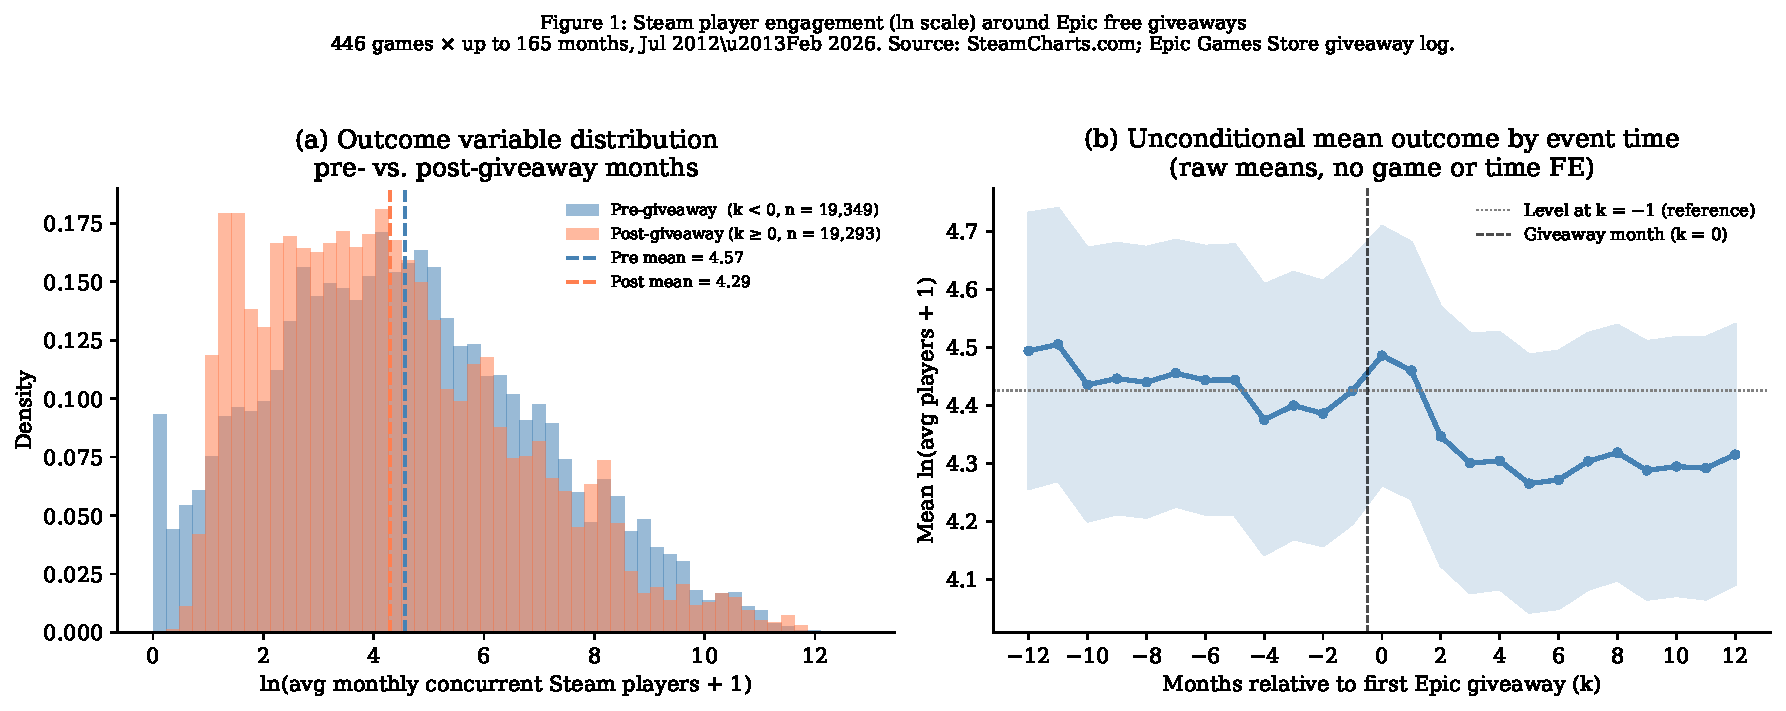
\includegraphics[width=0.88\linewidth]{../output/fig_outcome_histogram.pdf}
\caption{Steam player engagement (log scale) around Epic free giveaways.
  \textbf{Left:} Density histogram of $\ln(\texttt{avg\_players}+1)$ for pre-giveaway
  months ($k < 0$, blue) and post-giveaway months ($k \geq 0$, orange), pooled across
  all 446 games.
  \textbf{Right:} Unconditional mean (with 95\% CI) of the outcome by event-time
  $k \in [-12,12]$; the dashed vertical line marks the giveaway month ($k = 0$).}
\label{fig:outcome}
\end{figure}

\vspace{1em}

\begin{figure}[H]
\centering
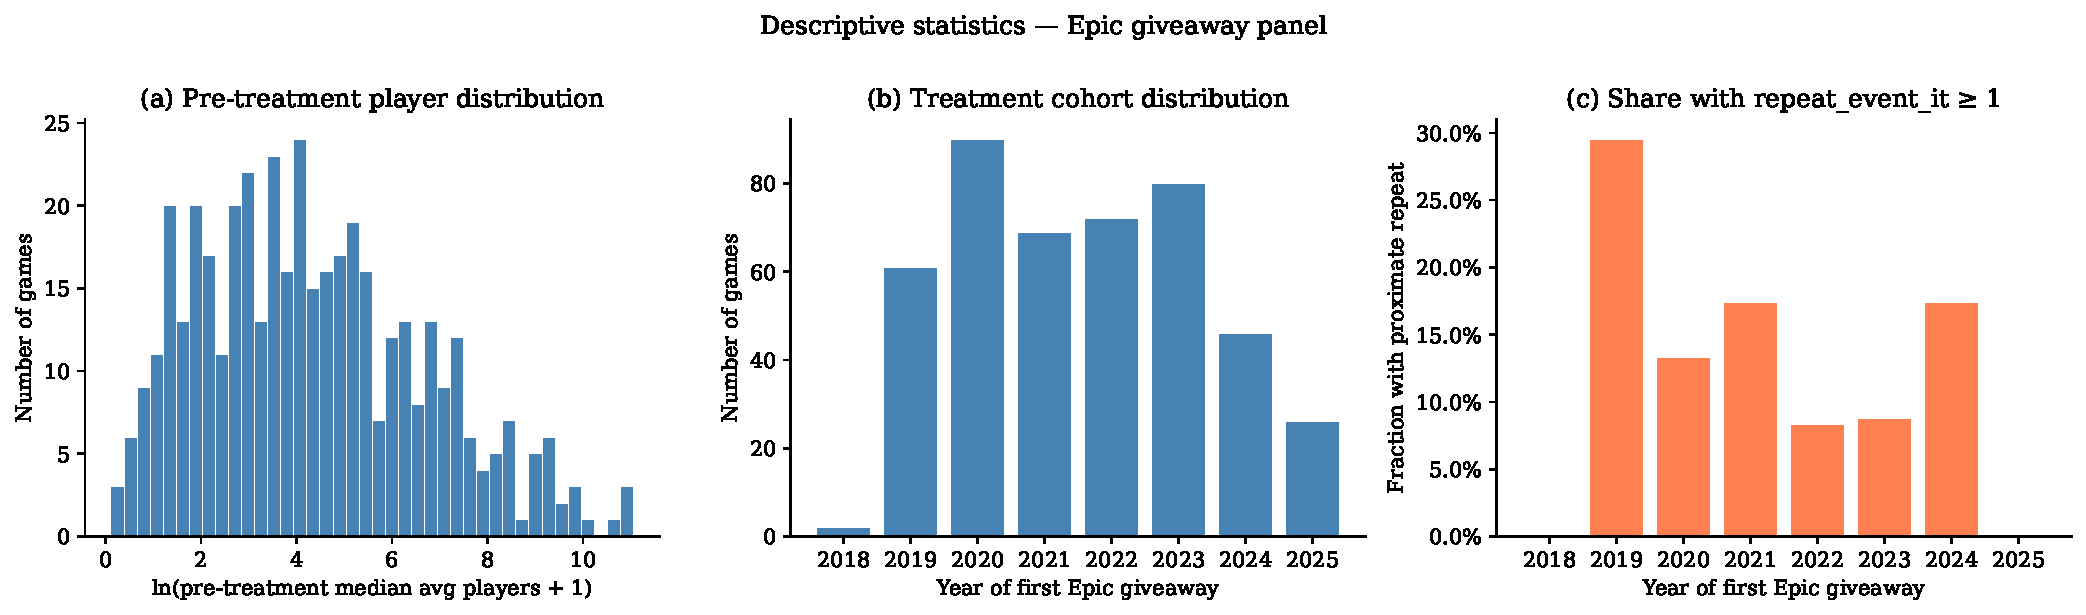
\includegraphics[width=0.88\linewidth]{../output/fig_descriptives.pdf}
\caption{Panel structure and descriptive statistics.
  \textbf{(a)} Histogram of $\ln(\text{pre-treatment median avg players} + 1)$
  across the 429 games with at least one pre-treatment observation (17 games
  whose first giveaway coincides with or precedes their earliest SteamCharts
  month have no defined pre-treatment median).
  \textbf{(b)} Number of games with first Epic giveaway in each calendar year
  (all 446 games).
  \textbf{(c)} Fraction of games in each cohort year that are ever flagged by
  the repeat-giveaway window indicator (i.e., received a second or later
  Epic giveaway during the panel, 63 games total; see Table~\ref{tab:epic_csv}).}
\label{fig:desc}
\end{figure}

\vspace{1em}

\begin{figure}[H]
\centering
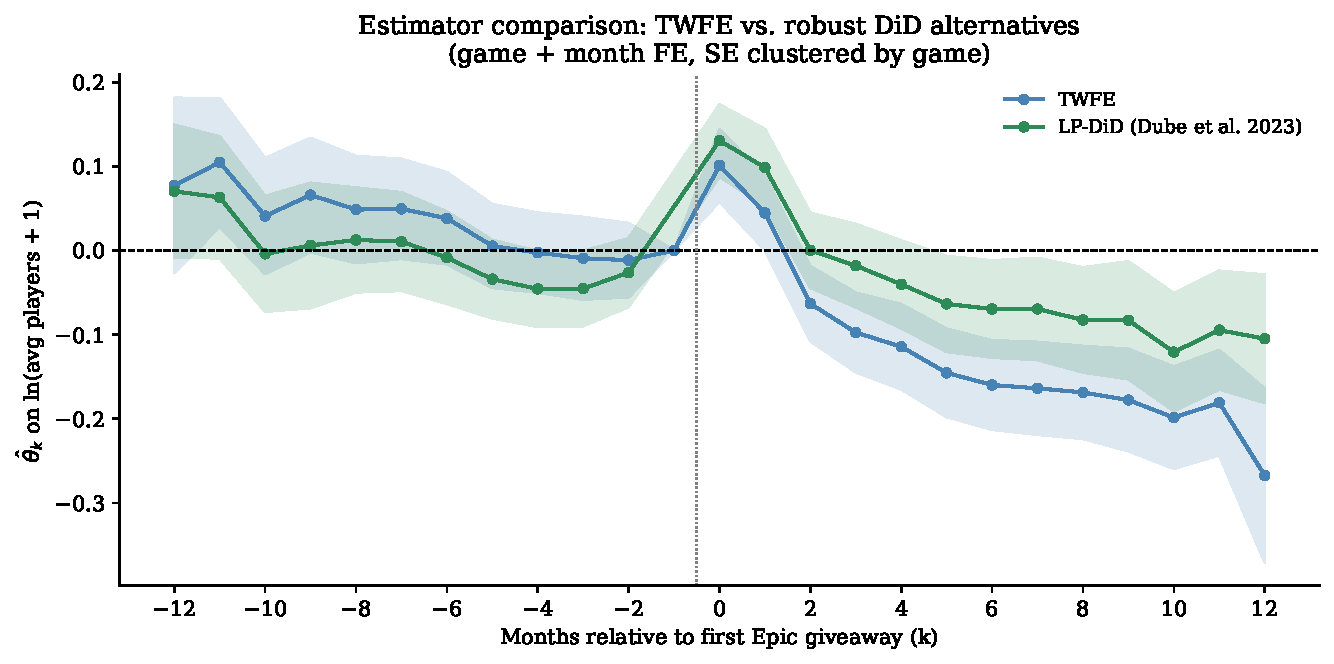
\includegraphics[width=0.82\linewidth]{../output/fig_estimator_comparison.pdf}
\caption{Event-study estimates: TWFE ($\hat{\theta}_k$, Eq.~\eqref{eq:pooled}),
  LP-DiD \citep{dube2023}, and stacked DiD \citep{cengiz2019}.
  Outcome: $\ln(\texttt{avg\_players}+1)$.
  TWFE uses game and calendar-month fixed effects; standard errors clustered by game.
  LP-DiD uses not-yet-treated controls at each period $k$ independently.
  Stacked DiD constructs cohort-specific balanced panels with not-yet-treated
  controls, regresses $\ln(\texttt{avg\_players}+1)$ on event-time dummies
  interacted with a treated indicator, absorbs unit-within-stack and
  stack-by-calendar-month fixed effects, and weights games in multiple stacks by
  $1/\text{number of stacks}$.
  All estimators share the same $[-12, 12]$ event window; shaded bands are
  95\% confidence intervals. Omitted category: $k = -1$.
  $N = 38{,}641$ game-month observations; 446 games.}
\label{fig:compare}
\end{figure}

\vspace{1em}

\begin{figure}[H]
\centering
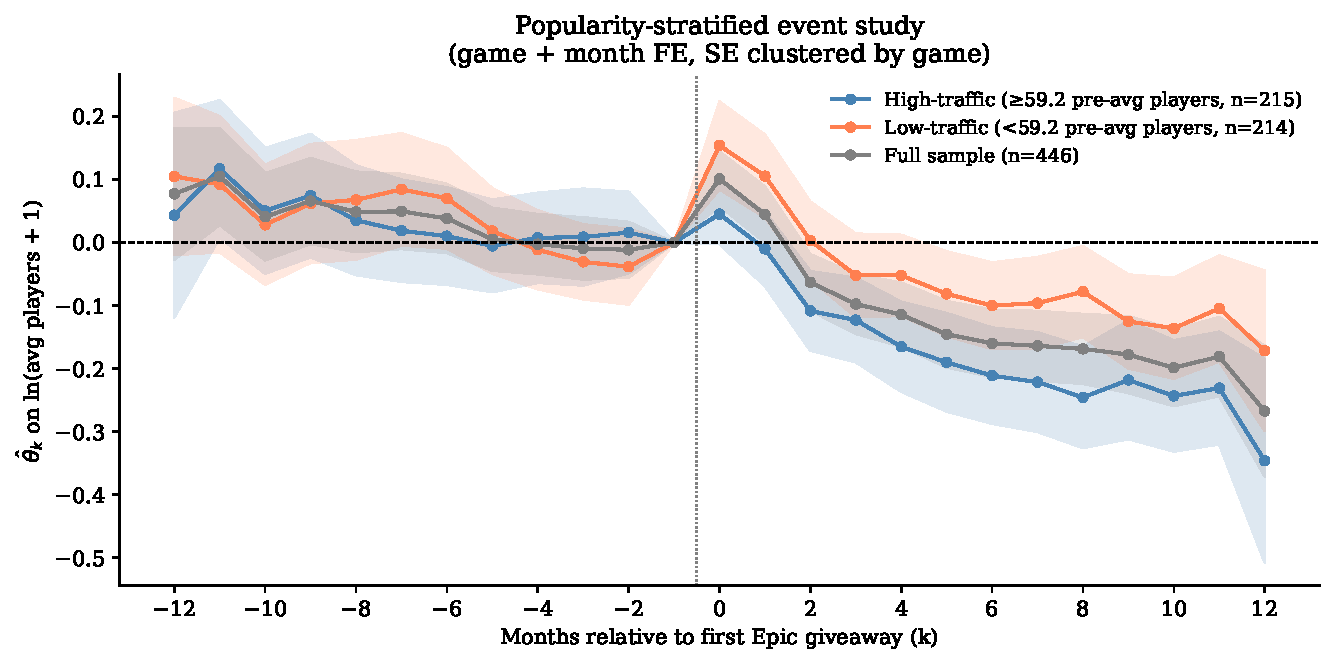
\includegraphics[width=0.88\linewidth]{../output/fig_event_study_popularity.pdf}
\caption{Event-study estimates by pre-treatment popularity. Outcome:
  $\ln(\texttt{avg\_players}+1)$. Split at the pre-treatment median (59.2 avg
  players/month): high-traffic ($N = 215$ games) and low-traffic
  ($N = 214$ games). 17 games with no pre-period observations are
  unclassified and enter only the pooled specification. Pre-trend joint Wald
  tests: high-traffic $\chi^2_{11} = 9.04$, $p = 0.618$; low-traffic
  $\chi^2_{11} = 20.82$, $p = 0.035$.}
\label{fig:popularity}
\end{figure}

\vspace{1em}

\begin{figure}[H]
\centering
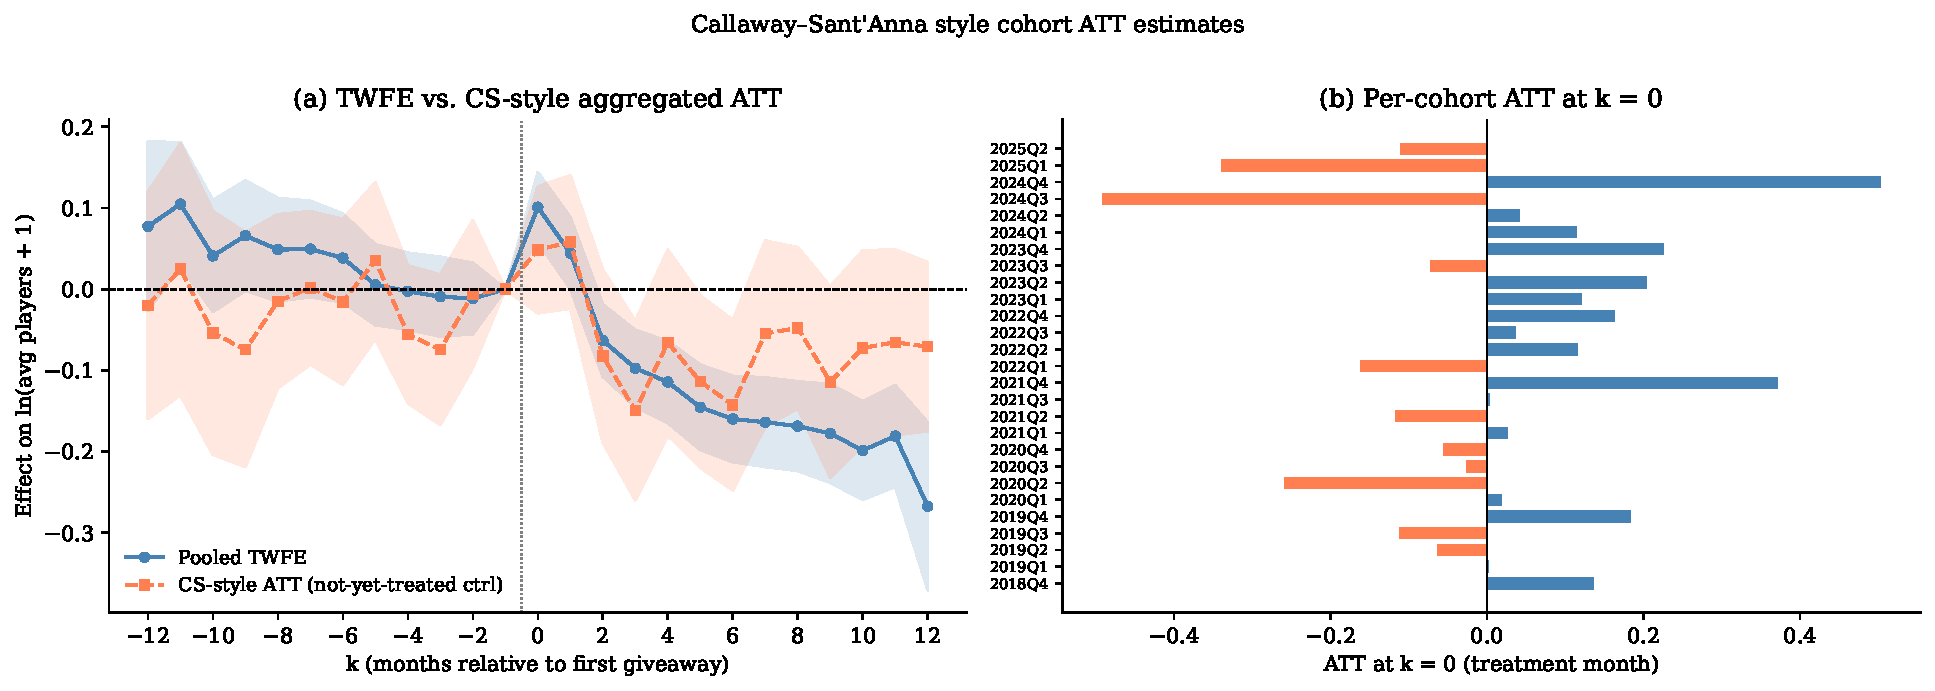
\includegraphics[width=0.82\linewidth]{../output/fig_cs_att.pdf}
\caption{Callaway--Sant'Anna cohort-aggregated ATT estimates. Outcome: $\ln(\texttt{avg\_players}+1)$.
  Not-yet-treated games serve as controls within each treatment-quarter cohort; estimates
  are aggregated across treatment-quarter cohorts weighted by cohort size.
  Omitted period: $k = -1$.}
\label{fig:csatt}
\end{figure}

\vspace{1em}

\begin{figure}[H]
\centering
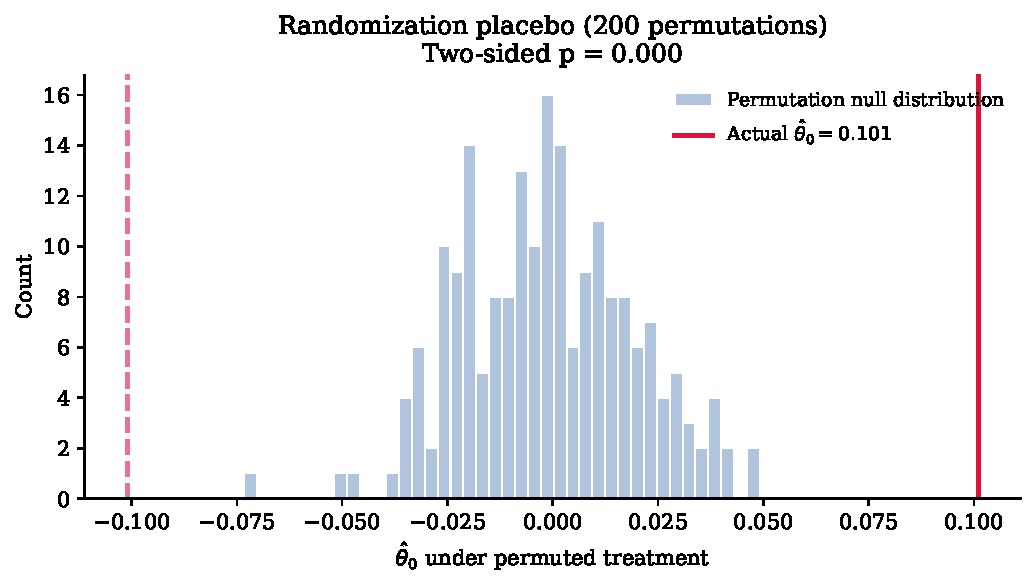
\includegraphics[width=0.72\linewidth]{../output/fig_randomization_placebo.pdf}
\caption{Randomization placebo test. Histogram of $|\hat{\theta}_0|$ from 200
  permutations of treatment dates (preserving the empirical distribution of treatment
  months). Red vertical line: actual estimate $|\hat{\theta}_0| = 0.101$. The 95th
  percentile of the permutation null is 0.038; empirical $p < 0.001$.}
\label{fig:placebo}
\end{figure}

\clearpage

% ═══════════════════════════════════════════════════════════════════════════
%  APPENDIX
% ═══════════════════════════════════════════════════════════════════════════

\appendix
\renewcommand{\thesection}{\Alph{section}}
\setcounter{section}{0}

\begin{center}
{\large\bfseries Appendix}\\[0.3em]
\end{center}

\vspace{1em}

\section{Clean-Sample Robustness Check}
\label{app:robustness}

Figure~\ref{fig:robustness} presents the pooled TWFE event-study on the clean
sample that drops all 30 games with a proximate repeat giveaway (within 12
months), leaving 416 single-event games. The coefficients are nearly identical
to the full-sample pooled TWFE (see Figure~\ref{fig:compare}), confirming that
repeat-giveaway contamination is not materially distorting the first-event
estimates.

\begin{figure}[H]
\centering
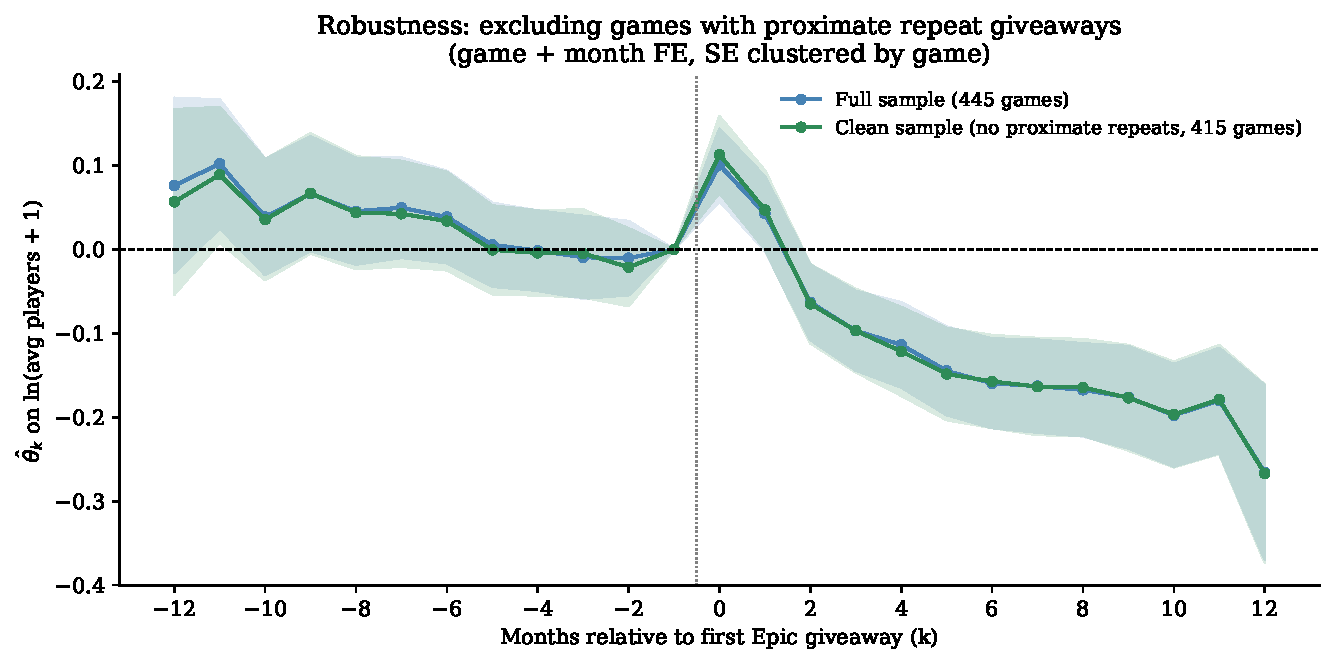
\includegraphics[width=0.82\linewidth]{../output/fig_event_study_robustness.pdf}
\caption{Clean-sample robustness check. Pooled TWFE re-estimated after dropping all 30
  games with a proximate repeat giveaway (within 12 months), leaving 416 games.
  Coefficients are virtually identical to the TWFE path in Figure~\ref{fig:compare}.}
\label{fig:robustness}
\end{figure}

\clearpage

\section{Holiday-Batch Robustness Check}
\label{app:holiday}

Dropping the 73 games whose first giveaway falls during one of Epic's five
December ``15 days of free games'' batches
leaves a 373-game sample of 32{,}108 game-months. Re-estimating the pooled
TWFE on this sample produces a treatment-month spike of $+0.109$ (compared
with $+0.101$ in the full sample) and a $k = 12$ estimate of $-0.258$
(compared with $-0.267$). Figure~\ref{fig:noholiday} overlays the no-holiday event-study
path on the full-sample TWFE estimates; the two paths are visually
indistinguishable. The advertising spike and the medium-run decline
therefore cannot be attributed to the holiday-batch media environment: they
persist in the same magnitude when those cohorts are removed.

\begin{figure}[H]
\centering
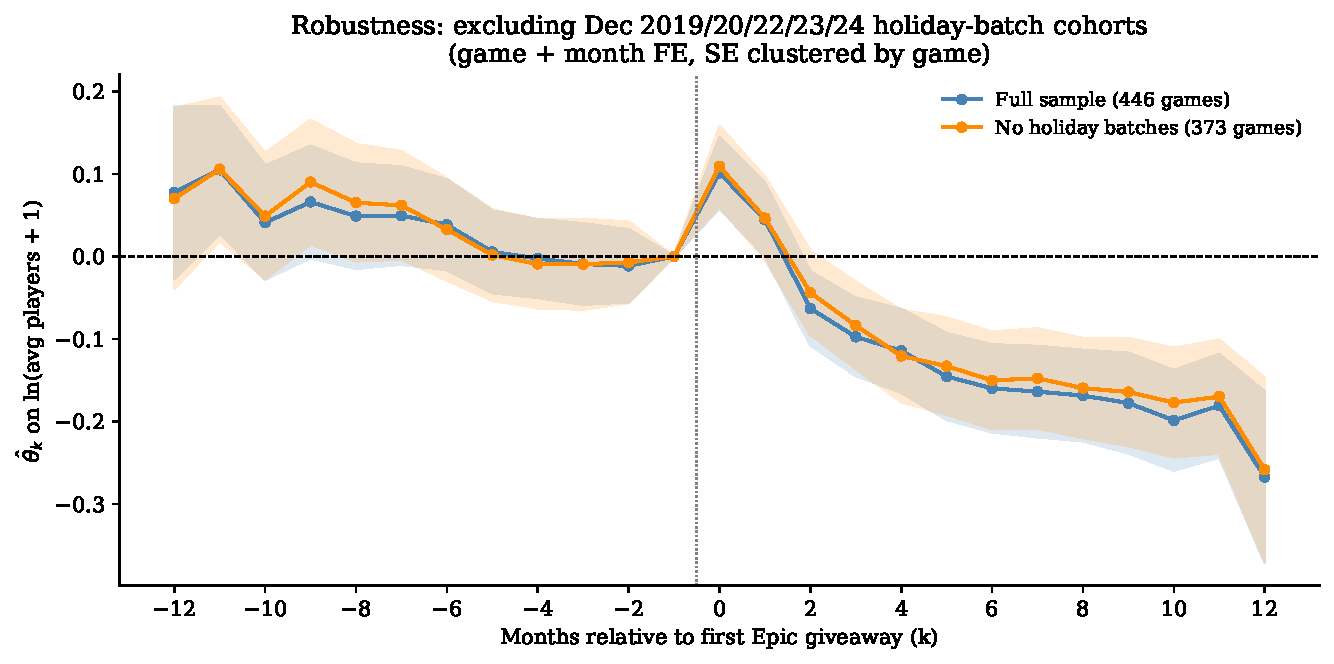
\includegraphics[width=0.82\linewidth]{../output/fig_event_study_no_holiday.pdf}
\caption{Holiday-batch robustness check. Pooled TWFE re-estimated after dropping
  the 73 games whose first giveaway falls in Epic's December holiday batches, leaving 373 games. Coefficients track the
  full-sample TWFE path closely.}
\label{fig:noholiday}
\end{figure}

\newpage

\section{Per-Cohort Event-Study Paths}
\label{app:cohort_paths}

Figure~\ref{fig:cohort_paths} overlays the full event-study path
$\widehat{\text{ATT}}(g,k)$ for each treatment cohort, coloured from early
(dark purple) to late (bright yellow) by quarter of first-giveaway exposure.
Lines are semi-transparent to reveal the density of trajectories; the thick
black dashed line reproduces the weighted CS aggregate from
Figure~\ref{fig:csatt}(a).
Individual cohort trajectories are highly dispersed and noisy---some spike
sharply upward at $k=0$, some show no visible jump, and a few drift in the
opposite direction. This chaos is expected: each cohort averages only a
handful of games with idiosyncratic lifecycle dynamics, so per-cohort ATTs
carry wide sampling error relative to the full-sample estimate. The
spike-and-decline pattern therefore emerges from averaging across cohorts
rather than from any individual cohort cleanly tracing it, which is why we
report the weighted CS aggregate in the main text and present the per-cohort
decomposition here primarily to document cohort heterogeneity.

\begin{figure}[H]
\centering
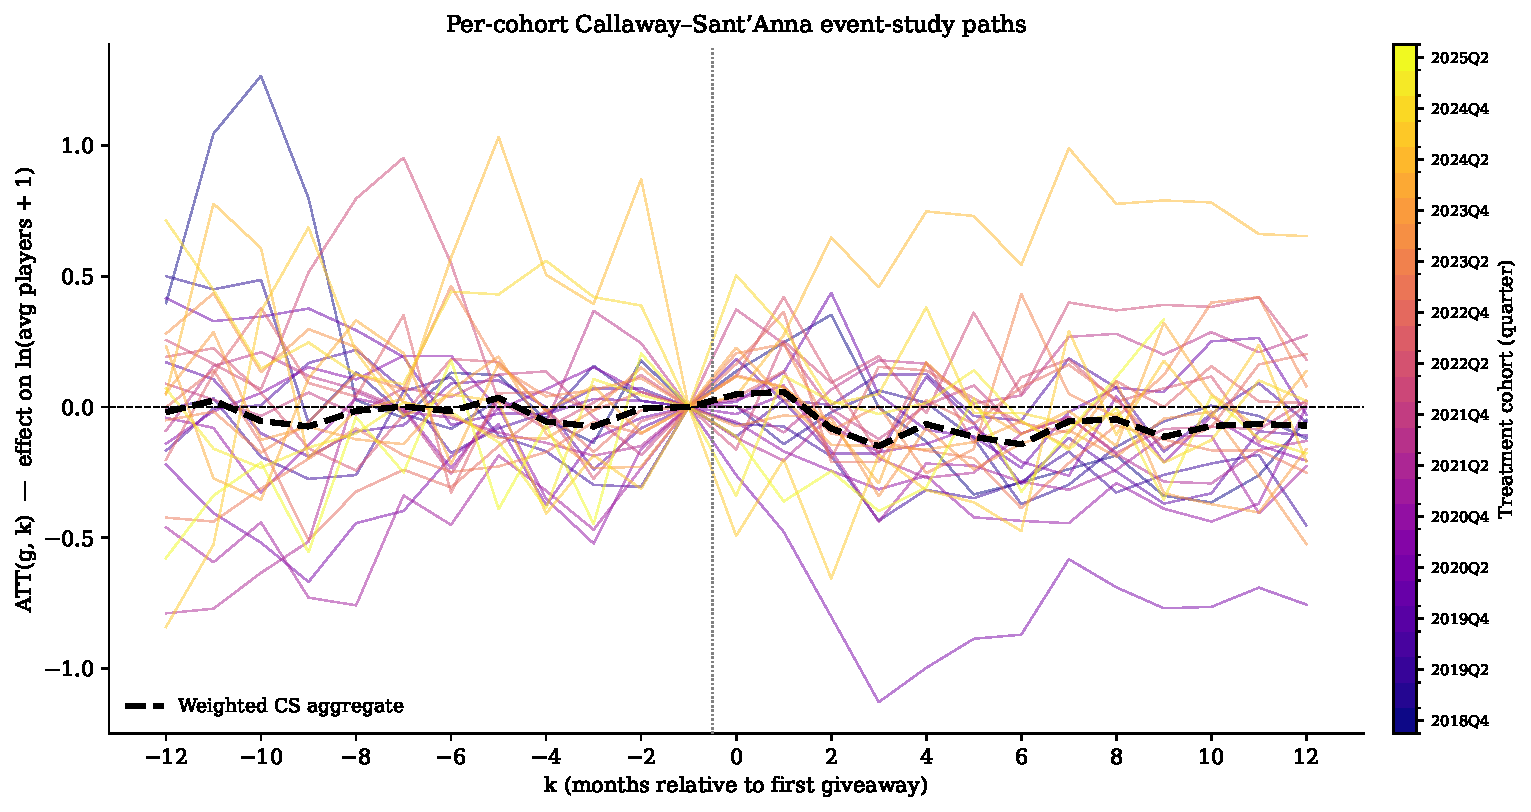
\includegraphics[width=0.88\linewidth]{../output/fig_cs_cohort_event_study.pdf}
\caption{Per-cohort Callaway--Sant'Anna event-study paths. Each thin line
  traces $\widehat{\text{ATT}}(g,k)$ for one treatment cohort $g$ across
  event times $k \in [-12,\,12]$; cohorts are coloured chronologically
  (early $\to$ late: purple $\to$ yellow).
  The thick black dashed line is the cohort-size-weighted CS aggregate.
  Vertical dotted line marks $k=-0.5$; horizontal dashed line marks zero.}
\label{fig:cohort_paths}
\end{figure}

\newpage

\section{Full TWFE Coefficient Table}
\label{app:coeftable}

Table~\ref{tab:fullcoefs} reports all 24 event-time coefficients from the pooled TWFE
specification (Equation~\eqref{eq:pooled}), including confidence intervals.

\begin{table}[H]
\centering\small
\caption{Full pooled TWFE event-study coefficients ($\hat{\theta}_k$)}
\label{tab:fullcoefs}
\begin{tabular}{rrcccc}
\toprule
$k$ & Estimate & SE & $p$-value & 2.5\% & 97.5\% \\
\midrule
$-12$ &  0.077 & 0.053 & 0.145 & $-0.027$ & 0.181 \\
$-11$ &  0.105 & 0.039 & 0.007 &    0.028 & 0.181 \\
$-10$ &  0.041 & 0.035 & 0.242 & $-0.028$ & 0.110 \\
$-9$  &  0.066 & 0.035 & 0.057 & $-0.002$ & 0.134 \\
$-8$  &  0.049 & 0.032 & 0.132 & $-0.015$ & 0.112 \\
$-7$  &  0.049 & 0.030 & 0.102 & $-0.010$ & 0.109 \\
$-6$  &  0.038 & 0.028 & 0.168 & $-0.016$ & 0.093 \\
$-5$  &  0.005 & 0.025 & 0.833 & $-0.044$ & 0.055 \\
$-4$  & $-0.003$ & 0.024 & 0.915 & $-0.050$ & 0.045 \\
$-3$  & $-0.009$ & 0.025 & 0.710 & $-0.058$ & 0.040 \\
$-2$  & $-0.011$ & 0.022 & 0.608 & $-0.055$ & 0.032 \\
$-1$  & 0 (ref) & --- & --- & --- & --- \\
\midrule
$0$  & $\mathbf{0.101}^{***}$ & 0.022 & $<$0.001 & 0.058 & 0.144 \\
$1$  & $0.045^{*}$ & 0.022 & 0.047 &  0.001 & 0.089 \\
$2$  & $-0.063^{**}$ & 0.023 & 0.005 & $-0.108$ & $-0.019$ \\
$3$  & $-0.097^{***}$ & 0.024 & $<$0.001 & $-0.145$ & $-0.050$ \\
$4$  & $-0.114^{***}$ & 0.026 & $<$0.001 & $-0.165$ & $-0.064$ \\
$5$  & $-0.145^{***}$ & 0.027 & $<$0.001 & $-0.198$ & $-0.093$ \\
$6$  & $-0.160^{***}$ & 0.027 & $<$0.001 & $-0.213$ & $-0.107$ \\
$7$  & $-0.164^{***}$ & 0.028 & $<$0.001 & $-0.219$ & $-0.109$ \\
$8$  & $-0.169^{***}$ & 0.028 & $<$0.001 & $-0.224$ & $-0.114$ \\
$9$  & $-0.178^{***}$ & 0.031 & $<$0.001 & $-0.238$ & $-0.117$ \\
$10$ & $-0.199^{***}$ & 0.031 & $<$0.001 & $-0.259$ & $-0.138$ \\
$11$ & $-0.181^{***}$ & 0.032 & $<$0.001 & $-0.243$ & $-0.119$ \\
$12$ & $-0.267^{***}$ & 0.053 & $<$0.001 & $-0.371$ & $-0.164$ \\
\bottomrule
\end{tabular}
\medskip

\noindent\small\textit{Notes:} Dependent variable: $\ln(\texttt{avg\_players}+1)$.
  TWFE, $N = 38{,}641$; game and calendar-month fixed effects;
  standard errors clustered by game.
  $R^2 = 0.884$; within $R^2 = 0.008$.
\end{table}

\clearpage

% ─────────────────────────── REFERENCES ────────────────────────────────────
\begin{thebibliography}{Callaway and Sant'Anna (2021)}
\setlength{\itemsep}{0.8em}

\bibitem[Callaway and Sant'Anna(2021)]{callaway2021}
Callaway, B.\ and Sant'Anna, P.H.C.\ (2021).
``Difference-in-Differences with Multiple Time Periods.''
\textit{Journal of Econometrics}, 225(2), 200--230.

\bibitem[Clarkson(2025)]{clarkson2025}
Clarkson, T.C.\ (2025).
``Essays on Platform Operations: Applications in Service Operations and Sustainability.''
Doctoral dissertation, Moore School of Business, University of South Carolina.
Retrieved from \url{https://scholarcommons.sc.edu/etd/8313}.

\bibitem[Dongre(2025)]{dongre2025}
Dongre, P.\ (2025).
``Epic Games Free Giveaway History 2018--2025.''
Kaggle dataset. Available at
\url{https://www.kaggle.com/datasets/prajwaldongre/epic-games-free-giveaway-history-20182025}
(accessed April 2026).

\bibitem[Dub\'{e} et al.(2023)]{dube2023}
Dub\'{e}, A., Girardi, D., Jord\`{a}, O., and Taylor, A.M.\ (2023).
``A Local Projections Approach to Difference-in-Differences Event Studies.''
NBER Working Paper No.\ 31184.

\bibitem[FRVR Blog(2026)]{frvr2026}
FRVR Blog (2026).
``Epic Game Store's Free Giveaways Just Cause a Huge Spike in Steam Sales,
Reveals New Blood CEO.''
\textit{FRVR Blog}, January 20, 2026.
Retrieved from \url{https://frvr.com/blog/epic-game-stores-free-giveaways-just-causes-a-huge-spike-in-steam-sales/}.


\bibitem[Cengiz et al.(2019)]{cengiz2019}
Cengiz, D., Dube, A., Lindner, A., and Zipperer, B.\ (2019).
``The Effect of Minimum Wages on Low-Wage Jobs.''
\textit{Quarterly Journal of Economics}, 134(3), 1405--1454.

\bibitem[Baker et al.(2022)]{bakerlarckerwang2022}
Baker, A.C., Larcker, D.F., and Wang, C.C.Y.\ (2022).
``How Much Should We Trust Staggered Difference-In-Differences Estimates?''
\textit{Journal of Financial Economics}, 144(2), 370--395.

\bibitem[Nabil and Ariatmanto(2025)]{nabil2025}
Nabil, M.\ and Ariatmanto, D.\ (2025).
``Analysis of User Satisfaction and Preferences in Choosing a Digital Game Platform
(Study Case: Steam vs Epic Games Store).''
\textit{G-Tech: Jurnal Teknologi Terapan}, 9(3), 1166--1175.

\bibitem[Reddit(2026)]{reddit2026}
r/Steam\ (2026).
``Epic Game Store's Free Giveaways Just Cause a Huge Spike in Steam Sales.''
Reddit, January 2026.
Retrieved from \url{https://www.reddit.com/r/Steam/comments/1qi94gk/epic_game_stores_free_giveaways_just_cause_a_huge/}.

\bibitem[Rochet and Tirole(2003)]{rochet2003}
Rochet, J.-C.\ and Tirole, J.\ (2003).
``Platform Competition in Two-Sided Markets.''
\textit{Journal of the European Economic Association}, 1(4), 990--1029.

\bibitem[Tud\'on(2022)]{tudon2022}
Tud\'on, J.\ (2022).
``Distilling Network Effects from Steam.''
\textit{Quantitative Marketing and Economics}, 20, 293--312.

\end{thebibliography}

\vspace{1em}
\noindent\textit{Note on AI usage: I used AI to assist with drafting and formatting this
document in \LaTeX.}

\end{document}
